%! TeX root = main.tex
\documentclass[fontsize=12pt,a4paper,oneside,DIV=calc, chapterprefix=true]{scrbook} % twoside for draft
\KOMAoptions{open=any}
\usepackage{tocloft}
\renewcommand{\cfttoctitlefont}{\rmfamily\bfseries\huge}
% Giảm khoảng cách trên/dưới tiêu đề MỤC LỤC
\renewcommand{\cftbeforetoctitleskip}{-0.5em}

% Encoding and fonts (pdfLaTeX)
\usepackage[T5]{fontenc}        % Vietnamese characters
\usepackage[utf8]{inputenc}     % UTF-8 input
\usepackage[vietnam]{babel}     % Vietnamese hyphenation & captions
\usepackage{newtxtext,newtxmath}% Times-like font with math support (better than mathptmx)

\usepackage{enumitem}           % Custom enumerate labels
\renewcommand{\contentsname}{{\rmfamily\bfseries MỤC LỤC}}
\addtokomafont{chapter}{\rmfamily\bfseries}
\addtokomafont{section}{\rmfamily}
\addtokomafont{subsection}{\rmfamily}
\addtokomafont{subsubsection}{\rmfamily}
\addtokomafont{paragraph}{\rmfamily}
\addtokomafont{subparagraph}{\rmfamily}
\addtokomafont{chapterentry}{\rmfamily\bfseries}


\addtokomafont{chapter}{\rmfamily\bfseries}
\addtokomafont{section}{\rmfamily\bfseries}
\addtokomafont{subsection}{\rmfamily}
\renewcommand{\contentsname}{\normalfont\bfseries MỤC LỤC}
\renewcommand{\cftchapfont}{\rmfamily\bfseries}
\renewcommand{\cftbeforetoctitleskip}{2em}
\renewcommand{\cftsecfont}{\rmfamily}
\renewcommand{\cftsubsecfont}{\rmfamily}
\renewcommand{\cftsubsubsecfont}{\rmfamily}

\usepackage{amsmath, amsfonts, amssymb, bm, tabularx}
\numberwithin{equation}{section}  % equations numbered by section

% Layout and formatting
\usepackage[paperheight=29.7cm, paperwidth=21cm, left=3cm, right=2cm, top=2.5cm, bottom=2.5cm]{geometry} % A4 with margins
% \usepackage[fontsize=13pt]{scrextend}  % Font size
\usepackage{indentfirst}              % Indent first paragraph
\setlength{\parindent}{1cm}           % Paragraph indent
% \setlength{\parskip}{6pt}             % Space between paragraphs
% \renewcommand{\baselinestretch}{1.2}  % Line spacing

% Graphics and figures
\usepackage{graphicx}
\usepackage{float}
\usepackage{tikz}
\usetikzlibrary{calc}

% Hyper reference
\usepackage[colorlinks=true, linkcolor=black, urlcolor=blue, citecolor=blue]{hyperref}

\usepackage{float}
\usepackage{subcaption} % loads the caption package
\usepackage{amssymb}
%\usepackage{babel}
\usepackage[utf8]{inputenc}
\inputencoding{latin1}
\inputencoding{utf8}
\usepackage{tabto}    
\usepackage{wrapfig}
\usepackage{lscape}
%\usepackage{tipa}
%\usepackage{amssymb}
 
%\usepackage{subcaption}
%\usepackage{booktabs}
\usepackage{amsmath}
%\usepackage{amssymb}
%\usepackage{amsfonts}
%\usepackage{ipa}
%\renewcommand{\rmdefault}{phv} % Arial
%\renewcommand{\sfdefault}{phv} % Arial
\usepackage{array}
\newcolumntype{P}[1]{>{\centering\arraybackslash}p{#1}}
\newcolumntype{M}[1]{>{\centering\arraybackslash}m{#1}}
\usepackage{fancyhdr}
\usepackage{multirow}
% \usepackage{algorithm2e}
\usepackage[unicode]{hyperref}
% \usepackage{tabularx}
\usepackage{cleveref}
\usepackage{amsmath,amssymb,amsfonts}
\usepackage{graphicx}
\usepackage{booktabs}
\usepackage{algorithm}
\usepackage{algorithmic}
\usepackage{hyperref}

% \usepackage{amsthm}
% \usepackage{amsmath, amssymb, amsfonts, amsthm}
% \usepackage{graphicx}
% \usepackage{booktabs}
% \usepackage{tabularx}
% \usepackage{adjustbox}
% \usepackage{float}
% \usepackage{caption}
% \usepackage{algorithm}
% \usepackage{algorithmic}
% \usepackage{algpseudocode}
% \usepackage{algorithm2e}
% \usepackage{hyperref}
 
\theoremstyle{definition}
\newtheorem{example}{Ví dụ}[section]

\usepackage{pgfplots}
\pgfplotsset{compat=1.18}

\theoremstyle{plain}
\newtheorem{theorem}{Định lý}[section]

\theoremstyle{remark}
\newtheorem{remark}{Nhận xét}

\theoremstyle{definition}
\newtheorem{definition}{Định nghĩa}[section]
\newtheorem{corollary}{Hệ quả}[section]





\begin{document}

% Section formatting
\setcounter{secnumdepth}{4}
% \titleformat*{\section}{\fontsize{20pt}{24pt}\selectfont \bfseries}
% \titlespacing*{\section}{0pt}{0pt}{10pt}



% Custom cover page
\thispagestyle{empty}


\begin{center}
  \vspace{1.2cm}
  \textbf{ĐẠI HỌC QUỐC GIA HÀ NỘI} \\[0.2cm]
  \textbf{\fontsize{14pt}{17pt}\selectfont TRƯỜNG ĐẠI HỌC KHOA HỌC TỰ NHIÊN}

  \vspace{1.2cm}
  
\includegraphics[width=0.18\textwidth]{figures/hus_logo.jpg}

  \vspace{1.2cm}
  {\bfseries\fontsize{35pt}{33pt}\selectfont BÁO CÁO CUỐI KỲ}

  \vspace{0.5cm}
  {\bfseries\fontsize{22pt}{26pt}\selectfont Chuyên Đề Đại Số}

  \vspace{0.8cm}
  \parbox{\dimexpr\textwidth - 1.2cm\relax}{
    \centering
    \textbf{\fontsize{18pt}{25pt}\selectfont
      Đề tài: Nghiệm của phương trình một nghiệm và\\
      Phương pháp lặp trong ma trận đại số}
  }

  \vspace{1.6cm}
  \renewcommand{\arraystretch}{1.2}
  \begin{tabular}{@{}l l@{}}
    \textbf{\fontsize{14pt}{17pt}Hà Thanh Hương}         & \textbf{\fontsize{14pt}{17pt}- 23007944} \\[-0.2em]
    \textbf{\fontsize{14pt}{17pt}Nguyễn Thị Minh Phượng} & \textbf{\fontsize{14pt}{17pt}- 23007937} \\[-0.2em]
    \textbf{\fontsize{14pt}{17pt}Lý Đức Trung}           & \textbf{\fontsize{14pt}{17pt}- 23007933} \\[-0.2em]
    \textbf{\fontsize{14pt}{17pt}Nguyễn Thị Ngọc Uyên}   & \textbf{\fontsize{14pt}{17pt}- 23007930}
  \end{tabular}
  \renewcommand{\arraystretch}{1}

  \vspace{0.8cm}
  \textbf{Chuyên ngành: Khoa học Dữ liệu} \\

  \vspace{1.6cm}
  \textbf{Giảng viên hướng dẫn:} \textbf{TS. Nguyễn Trung Hiếu}

  \vspace{2cm}
  \fontsize{14pt}{17pt}\selectfont Hà Nội, 11/2025
\end{center}

\cleardoublepage
  

\clearpage
\thispagestyle{empty} % Ẩn header/footer nếu cần

\vspace*{\fill} % Đẩy nội dung xuống giữa trang
{\centering \LARGE \textbf{LỜI CẢM ƠN} \par}
\vspace{2em}
Bài tiểu luận cuối kỳ này được hoàn thành dưới sự hướng dẫn của thầy Nguyễn Trung Hiếu. Chúng em xin bày tỏ lòng biết ơn sâu sắc tới thầy vì sự định hướng đề tài trong quá trình học tập môn học này.

Trong quá trình làm bài tiểu luận này, do kiến thức còn hạn chế nên chúng em không tránh khỏi những thiếu sót. Chúng em mong nhận được những ý kiến đóng góp của thầy và các bạn để có thể rút ra kinh nghiệm, hoàn thiện và phát triển đề tài hơn.

Chúng em xin chân thành cảm ơn!
\vspace{5cm}
\vspace*{\fill} % Đẩy phần dưới lên để căn giữa


\clearpage % ✅ tự động sang trang sau khi kết thúc Lời cảm ơn
% \vspace{-2cm}
\tableofcontents

\fancyhead{}  % Clears all page headers and footers
% \rhead{\thepage}  % Sets the right side header to show the page number
% \lhead{}  % Clears the left side page header
%\fancyfoot[positions]{footer}
\renewcommand{\footrulewidth}{0.4pt}

\pagestyle{fancy}  

% Chapter 0
\chapter*{Giới thiệu}

Trong lĩnh vực phân tích số, việc tìm nghiệm của phương trình và hệ phương trình đóng vai trò quan trọng trong nhiều bài toán khoa học và kỹ thuật. Các phương pháp giải phương trình một biến và hệ tuyến tính không chỉ cung cấp công cụ tính toán mà còn giúp hiểu rõ bản chất hội tụ và sai số của các thuật toán.

Tiểu luận này tập trung vào các nội dung sau:
\begin{itemize}
    \item \textbf{Phương pháp giải phương trình một biến:} Bao gồm \emph{Phương pháp chia đôi}, \emph{Lặp điểm cố định}, \emph{Phương pháp Newton và các mở rộng}, phân tích sai số và kỹ thuật tăng tốc hội tụ.
    \item \textbf{Phương pháp lặp cho hệ tuyến tính:} Bao gồm \emph{Jacobi}, \emph{Gauss-Seidel}, các kỹ thuật thư giãn và tinh chỉnh sai số.
\end{itemize}

Mục tiêu của bài viết là so sánh đặc điểm, ưu nhược điểm và điều kiện hội tụ của các phương pháp trên, đồng thời minh họa bằng ví dụ thực tế và phân tích sai số.



% Chapter 1

\vspace*{1em}
\chapter{Phương Pháp Giải Phương Trình Một Biến}

Trong nhiều bài toán thực tế, việc tìm nghiệm của phương trình một biến đóng vai trò quan trọng trong mô hình hóa và phân tích. Một ví dụ điển hình là mô hình tăng trưởng dân số, trong đó số lượng quần thể $N(t)$ thay đổi theo thời gian $t$ và được mô tả bởi phương trình vi phân:
\[
\frac{dN(t)}{dt} = \lambda N(t),
\]
với nghiệm:
\[
N(t) = N_0 e^{\lambda t},
\]
trong đó $N_0$ là dân số ban đầu và $\lambda$ là tỷ lệ sinh.

\begin{center}
\begin{tikzpicture}
\begin{axis}[
    width=10cm,
    height=7cm,
    xlabel={Tỷ lệ sinh $\lambda$},
    ylabel={Dân số (nghìn)},
    xmin=0, xmax=1.2,
    ymin=1000, ymax=3200,
    domain=0:1,
    samples=100,
    axis lines=middle,
    xtick={0,0.5,1},
    ytick={1000,1435,1564,2000,3000},
    yticklabels={1000,1435,1564,2000,3000},
    xlabel style={at={(axis description cs:1,0)},anchor=west},
    ylabel style={at={(axis description cs:0,1)},anchor=south},
]
% Vẽ đường cong N(λ) = 1000 e^x + (435/x)(e^x - 1)
\addplot[blue, thick] {1000*exp(x) + (435/x)*(exp(x)-1)};
% Ghi chú công thức
\node at (axis cs:0.6,2200) {$N(\lambda)=1000e^{\lambda}+\dfrac{435}{\lambda}(e^{\lambda}-1)$};
% Đường ngang tại 1564 và 1435
\draw[dashed] (axis cs:0,1564) -- (axis cs:1,1564);
\draw[dashed] (axis cs:0,1435) -- (axis cs:1,1435);
\end{axis}
\end{tikzpicture}
\end{center}


Khi có thêm yếu tố nhập cư với tốc độ không đổi $v$, phương trình trở thành:
\[
\frac{dN(t)}{dt} = \lambda N(t) + v,
\]
với nghiệm:
\[
N(t) = N_0 e^{\lambda t} + \frac{v}{\lambda}(e^{\lambda t} - 1).
\]

Trong thực tế, để xác định $\lambda$ từ dữ liệu quan sát, ta phải giải phương trình phi tuyến:
\[
1{,}564{,}000 = 1{,}000{,}000 e^{\lambda} + \frac{435{,}000}{\lambda}(e^{\lambda} - 1).
\]

Phương trình này không thể giải tường minh, do đó cần sử dụng các phương pháp số như \textit{phương pháp chia đôi}, \textit{lặp điểm cố định} hoặc \textit{phương pháp Newton} để tìm nghiệm gần đúng. Đây chính là lý do các kỹ thuật giải phương trình một biến trở thành công cụ thiết yếu trong phân tích số và ứng dụng thực tế.


\section{Phương pháp Chia Đôi (Bisection Method)}
\label{sec:bisection_method}

Trong chương này, chúng ta xem xét một trong những vấn đề cơ bản nhất của xấp xỉ số,
đó là \textit{bài toán tìm nghiệm}. Bài toán liên quan đến việc tìm một \textit{nghiệm}
của phương trình dạng $f(x)=0$ đối với một hàm $f$ cho trước. Một nghiệm của phương trình này
còn được gọi là một \textit{zero} của hàm $f$.

Bài toán tìm nghiệm xấp xỉ đã được biết đến từ thời Babylon cổ đại. Ví dụ,
họ đã xấp xỉ $\sqrt{2}$ đến độ chính xác $10^{-5}$. 

%---------------------------------------------------------
\subsection{Kỹ thuật Chia Đôi}
\label{subsec:bisection_technique}

Kỹ thuật này dựa trên \textit{Định lý Giá trị Trung gian (Intermediate Value Theorem)}
và được gọi là \textit{phương pháp chia đôi (bisection)} hoặc \textit{binary-search}.

Giả sử $f$ liên tục trên khoảng $[a,b]$, và $f(a)f(b) < 0$, khi đó tồn tại $p \in (a,b)$
sao cho $f(p)=0$.

Đặt $a_1=a$, $b_1=b$ và
\[
p_1 = \frac{a_1 + b_1}{2}.
\]

\begin{itemize}
    \item Nếu $f(p_1)=0$, khi đó nghiệm $p=p_1$.
    \item Nếu $f(p_1) \neq 0$:
        \begin{itemize}
            \item Nếu $f(a_1)$ và $f(p_1)$ cùng dấu, đặt $a_2=p_1$, $b_2=b_1$.
            \item Nếu trái dấu, đặt $a_2=a_1$, $b_2=p_1$.
        \end{itemize}
\end{itemize}

Tiếp tục quy trình đối với khoảng $[a_2,b_2]$.

\begin{figure}[!h]
\centering
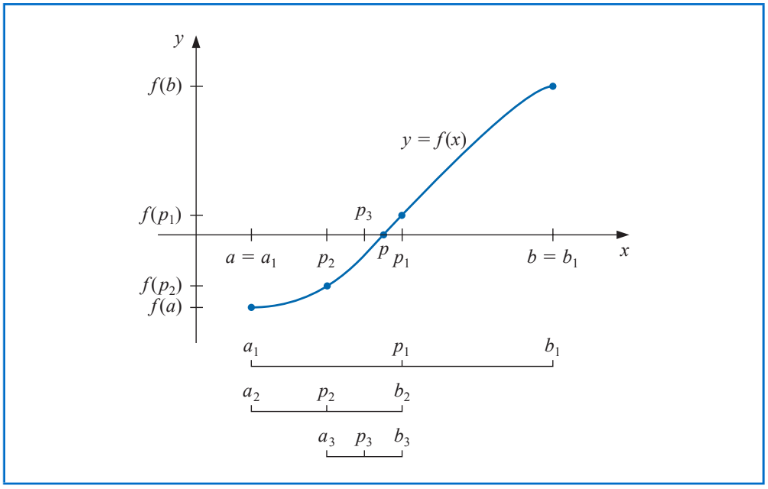
\includegraphics[width=0.65\linewidth]{figures/bisect_diagram_placeholder.png}
\caption{Minh họa phương pháp chia đôi.}
\label{fig:bisection_figure1}
\end{figure}

%---------------------------------------------------------
\subsection{Thuật toán Chia Đôi}
\label{subsec:bisection_algorithm}

\begin{algorithm}
\caption{Thuật toán Chia Đôi}
\label{alg:bisection}
\begin{algorithmic}[1]
\Require $a,b$ sao cho $f(a)f(b) < 0$, sai số $TOL$, số lặp tối đa $N_0$
\Ensure Nghiệm xấp xỉ $p$
\State $i \gets 1$
\State $FA \gets f(a)$
\While {$i \le N_0$}
    \State $p \gets a + \frac{b-a}{2}$
    \State $FP \gets f(p)$
    \If {$FP = 0$ or $\frac{b-a}{2} < TOL$}
        \Return $p$
    \EndIf
    \State $i \gets i+1$
    \If {$FA \cdot FP > 0$}
        \State $a \gets p$
        \State $FA \gets FP$
    \Else
        \State $b \gets p$
    \EndIf
\EndWhile
\Return {``Thất bại sau $N_0$ lặp.''}
\end{algorithmic}
\end{algorithm}

\subsection*{Các tiêu chí dừng bổ sung}
\label{subsec:additional_stopping}

Trong Bước~4 của Thuật toán~\ref{alg:bisection}, hoặc trong bất kỳ kỹ thuật lặp nào
được trình bày trong chương này, ta có thể áp dụng các tiêu chí dừng thay thế.
Ví dụ, ta có thể chọn một sai số $\varepsilon > 0$ và sinh ra dãy
$p_1, p_2, \dots, p_n$ cho đến khi thỏa mãn một trong các điều kiện sau:

\begin{align}
|p_n - p_{n-1}| &< \varepsilon, \label{eq:stop_a}\\[6pt]
\frac{|p_n - p_{n-1}|}{|p_n|} &< \varepsilon, \quad p_n \neq 0, \label{eq:stop_b}\\[6pt]
|f(p_n)| &< \varepsilon. \label{eq:stop_c}
\end{align}

Tuy nhiên, trong thực tế, một số khó khăn có thể phát sinh khi sử dụng riêng lẻ
bất kỳ tiêu chí dừng nào ở trên. Chẳng hạn, tồn tại các dãy $\{p_n\}_{n=1}^{\infty}$
mà sai khác $p_n - p_{n-1}$ tiến dần về 0, nhưng bản thân dãy lại \emph{diverge}
(không hội tụ). (Xem Bài tập~\ref{ex:exercise17}.) Ngoài ra, cũng có thể xảy ra trường hợp
giá trị $f(p_n)$ rất nhỏ trong khi khoảng cách $p_n$ đến nghiệm thực sự $p$ vẫn khác biệt đáng kể.

Khi không có thông tin bổ sung về độ lớn tuyệt đối hoặc tương đối của $p$, tiêu chí
tương đối \eqref{eq:stop_b} thường được xem là tốt hơn, vì nó gần nhất với ý nghĩa
sai số tương đối trong thực tế tính toán.

\subsection*{Giới hạn số vòng lặp}
\label{subsec:max_iterations}

Khi sử dụng máy tính để tạo xấp xỉ, việc đặt ra \textit{số vòng lặp tối đa} (iteration limit)
là một thực hành tốt. Điều này loại bỏ khả năng rơi vào vòng lặp vô hạn do sai sót trong việc
kiểm tra điều kiện dừng hoặc lập trình sai. Điều này đã được thực hiện trong Bước~2 của
Thuật toán~\ref{alg:bisection}, nơi giá trị $N_0$ được thiết lập và thủ tục sẽ dừng nếu
$i > N_0$.

\subsection*{Lựa chọn khoảng ban đầu}
\label{subsec:initial_interval}

Lưu ý rằng để bắt đầu Thuật toán Chia Đôi, đoạn $[a,b]$ phải thỏa $f(a)f(b) < 0$.
Ở mỗi bước, độ dài của đoạn chứa nghiệm giảm đi một hệ số $2$; do đó, việc chọn
đoạn ban đầu càng nhỏ càng tốt là điều có lợi.

Ví dụ, xét hàm:
\[
f(x) = 2x^3 - x^2 + x - 1.
\]

Ta có:
\[
f(-4)\cdot f(4) < 0
\quad\text{và}\quad
f(0)\cdot f(1) < 0.
\]

Do đó, có thể bắt đầu Thuật toán Chia Đôi trên đoạn $[-4,4]$ hoặc trên $[0,1]$.
Nếu xét đoạn $[0,1]$ thay vì $[-4,4]$, số vòng lặp cần thiết để đạt cùng độ chính xác
sẽ giảm đi khoảng $\log_2(8) = 3$ bước (tương ứng việc rút nhỏ đoạn ban đầu).

\label{subsec:example1}

\begin{example}
Xét phương trình
\[
f(x) = x^3 + 4x^2 - 10 = 0.
\]
Chứng minh rằng phương trình có nghiệm trong khoảng $[1,2]$ và sử dụng
phương pháp chia đôi (Bisection) để tìm nghiệm xấp xỉ với độ chính xác
ít nhất $10^{-4}$.
\end{example}

\paragraph*{Bước 1: Chứng minh tồn tại nghiệm.}
Ta có
\[
f(1) = 1^3 + 4(1)^2 - 10 = -5 < 0,
\qquad
f(2) = 2^3 + 4(2)^2 - 10 = 14 > 0.
\]
Vì $f(1)\cdot f(2) < 0$ nên theo Định lý Giá trị Trung gian,
tồn tại ít nhất một nghiệm $p \in (1,2)$.

\paragraph*{Bước 2: Áp dụng phương pháp chia đôi.}
Ta bắt đầu với $a_1 = 1$, $b_1 = 2$ và tính trung điểm
\[
p_1 = \frac{a_1 + b_1}{2} = 1.5.
\]

Sau đó ta kiểm tra dấu $f(a_n)$ và $f(p_n)$
để xác định khoảng con chứa nghiệm tại mỗi bước.

\paragraph*{Bảng tính lặp.}

\begin{table}[!h]
\centering
\caption{Các bước lặp của phương pháp chia đôi cho Ví dụ~\ref{subsec:example1}.}
\label{tab:example1-bisection}
\begin{tabular}{cccc}
\toprule
$n$ & $a_n$ & $b_n$ & $p_n$ \\
\midrule
1  & 1.0000       & 2.0000       & 1.5000 \\
2  & 1.0000       & 1.5000       & 1.2500 \\
3  & 1.2500       & 1.5000       & 1.3750 \\
4  & 1.2500       & 1.3750       & 1.3125 \\
5  & 1.3125       & 1.3750       & 1.34375 \\
6  & 1.34375      & 1.3750       & 1.359375 \\
7  & 1.359375     & 1.3750       & 1.3671875 \\
8  & 1.359375     & 1.3671875    & 1.36328125 \\
9  & 1.359375     & 1.36328125   & 1.361328125 \\
10 & 1.361328125  & 1.36328125   & 1.3623046875 \\
11 & 1.361328125  & 1.3623046875 & 1.36181640625 \\
12 & 1.36181640625 & 1.3623046875 & 1.362060546875 \\
13 & 1.36181640625 & 1.362060546875 & 1.3619384765625 \\
\bottomrule
\end{tabular}
\end{table}

\paragraph*{Bước 3: Kiểm tra tiêu chí dừng.}
Độ dài khoảng sau $n$ bước bằng
\[
b_n - a_n = \frac{2 - 1}{2^{n-1}} = \frac{1}{2^{n-1}}.
\]
Sai số tuyệt đối được chặn bởi
\[
|p - p_n| \le \frac{b_n - a_n}{2} = \frac{1}{2^n}.
\]

Tại $n = 13$,
\[
\frac{1}{2^{13}} = \frac{1}{8192} \approx 1.2207\times10^{-4} < 10^{-4},
\]
do đó sai số đã nhỏ hơn yêu cầu.

\paragraph*{Kết luận.}
Phương trình $f(x)=0$ có nghiệm trong $(1,2)$ và phương pháp chia đôi
cho xấp xỉ nghiệm:
\[
p \approx 1.36194,
\]
với sai số nhỏ hơn $10^{-4}$.

\begin{theorem}
\label{thm:bisection_convergence}
Giả sử $f$ liên tục trên đoạn $[a,b]$ và $f(a)\cdot f(b) < 0$. Phương pháp Chia Đôi
(Bisection) sinh ra dãy $\{p_n\}_{n=1}^{\infty}$ xấp xỉ nghiệm $p$ của phương trình
$f(x)=0$ sao cho
\[
|p_n - p| \le \frac{b - a}{2^n}, \qquad n \ge 1.
\]
\end{theorem}

\begin{proof}
Với mỗi $n \ge 1$, do phương pháp chia đôi bảo toàn dấu theo Định lý Giá trị Trung gian,
nghiệm $p$ luôn nằm trong khoảng $(a_n,b_n)$, nơi $b_n - a_n = \dfrac{1}{2^{\,n-1}}(b-a)$.

Vì $p_n$ là trung điểm khoảng $[a_n,b_n]$, nên
\[
|p_n - p| \le \frac{1}{2}(b_n - a_n) = \frac{b-a}{2^n}.
\]

Do đó
\[
|p_{n} - p| \le \frac{b-a}{2^n}.
\]

Từ đây ta suy ra dãy $\{p_n\}$ hội tụ về $p$ với tốc độ hội tụ
\[
p_n = p + \mathcal{O}\!\left(\frac{1}{2^n}\right).
\]
\end{proof}

\noindent
Lưu ý rằng định lý trên chỉ đưa ra một \emph{chặn trên} cho sai số xấp xỉ,
và trong thực tế chặn này có thể khá bảo thủ. Ví dụ, trong
Ví dụ~\ref{subsec:example1}, ta chỉ đảm bảo rằng
\[
|p - p_{9}| \le \frac{2-1}{2^9} = \frac{1}{512} \approx 2\times 10^{-3},
\]
nhưng sai số thực tế nhỏ hơn nhiều:
\[
|\,p - p_{9}\,| = |\,1.365230013 - 1.365234375\,|
    \approx 4.4\times 10^{-6}.
\]










\section{Phương pháp Lặp Điểm Cố Định (Fixed-Point Iteration)}
\label{sec:fixed_point_iteration}

Một \emph{điểm cố định} (fixed point) của một hàm là một số mà tại đó
giá trị của hàm không thay đổi sau khi được áp dụng.

\begin{definition}
\label{def:fixed_point}
Một số $p$ được gọi là \emph{điểm cố định} của hàm $g$ nếu
\[
g(p) = p.
\]
\end{definition}

Trong mục này, chúng ta xem xét bài toán tìm nghiệm của các hàm dưới dạng điểm cố định,
và mối liên hệ giữa bài toán điểm cố định và bài toán tìm nghiệm dạng $f(x)=0$.

Trên thực tế, hai lớp bài toán này là \emph{tương đương} theo các ý sau:

\begin{itemize}
    \item Nếu ta có bài toán tìm nghiệm $f(p)=0$, ta có thể xây dựng
    một hàm $g$ sao cho $p$ là điểm cố định:
    \[
    g(x) = x - f(x)
    \qquad \text{hoặc} \qquad
    g(x) = x + 3f(x),
    \]
    hay nhiều dạng khác.
    \item Ngược lại, nếu một hàm $g$ có điểm cố định $p$, thì hàm
    \[
    f(x) = x - g(x)
    \]
    sẽ có nghiệm tại $p$.
\end{itemize}

Như vậy, thay vì giải phương trình $f(x)=0$, ta có thể chuyển sang bài toán
tìm điểm cố định $g(x)=x$ — đôi khi đơn giản và dễ phân tích hơn.

\begin{remark}
Mặc dù các kỹ thuật tìm nghiệm thường được trình bày dưới dạng $f(x)=0$,
dạng điểm cố định $g(x)=x$ giúp xây dựng các phương pháp lặp mạnh và tinh tế hơn.
Ý tưởng nền tảng được hình thức hóa bởi nhà toán học người Hà Lan
L. E. J. Brouwer (1882–1962) vào đầu thế kỷ XX.
\end{remark}

Để sử dụng dạng này hiệu quả, chúng ta cần:
\begin{enumerate}
    \item Nhận biết khi nào một hàm $g$ có điểm cố định;
    \item Xem xét cách xấp xỉ điểm cố định $p$ với độ chính xác chỉ định.
\end{enumerate}

\begin{theorem}
\label{thm:fixed_point_existence_uniqueness}
Giả sử $g$ là hàm liên tục trên đoạn $[a,b]$ và $g(x) \in [a,b]$ với mọi $x \in [a,b]$.
Khi đó:
\begin{enumerate}
    \item Hàm $g$ tồn tại ít nhất một điểm cố định trong $[a,b]$.
    \item Nếu, thêm vào đó, $g$ khả vi trên $(a,b)$ và tồn tại hằng số dương $k<1$
    sao cho
    \[
    |g'(x)| \le k, \quad \forall x \in (a,b),
    \]
    thì điểm cố định trên là \emph{duy nhất} trong $[a,b]$.
\end{enumerate}
\end{theorem}

\begin{figure}[!h]
\centering
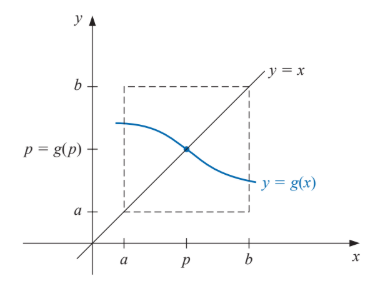
\includegraphics[width=0.6\linewidth]{figures/fixed_point_diagram_placeholder.png}
\caption{Minh họa điểm cố định của $g(x)$ trong $[a,b]$.}
\label{fig:fixed_point_figure}
\end{figure}

\begin{proof}

\textbf{(i)} Nếu $g(a) = a$ hoặc $g(b) = b$, ta đã có điểm cố định tại đầu mút.
Ngược lại, nếu
\[
g(a) > a \quad \text{và} \quad g(b) < b,
\]
xét hàm
\[
h(x) = g(x) - x.
\]
Do $g(x) \in [a,b]$, ta có $h(a) = g(a) - a > 0$ và $h(b) = g(b) - b < 0$.
Vì $h$ liên tục trên $[a,b]$, Định lý Giá trị Trung gian (IVT) suy ra tồn tại $p \in (a,b)$ sao cho
\[
h(p) = 0 \quad \Longleftrightarrow \quad g(p) = p.
\]
Do đó, $p$ là điểm cố định.

\bigskip
\textbf{(ii)} Giả sử tồn tại thêm điều kiện $|g'(x)| \le k < 1$ trên $(a,b)$.
Giả sử $p$ và $q$ đều là các điểm cố định trong $[a,b]$:
\[
g(p) = p, \qquad g(q) = q.
\]

Nếu $p \neq q$, áp dụng Định lý Giá trị Trung bình (MVT), tồn tại $\xi \in (a,b)$ sao cho
\[
\frac{g(p) - g(q)}{p - q} = g'(\xi).
\]
Do đó,
\[
|p - q|
= |g(p) - g(q)|
= |g'(\xi)|\,|p - q|
\le k\,|p - q|.
\]

Vì $0 \le k < 1$, biểu thức trên chỉ có thể xảy ra nếu $|p - q| = 0$, tức là $p=q$.

Suy ra điểm cố định là duy nhất.

\end{proof}

\subsection{Phương pháp Lặp Điểm Cố Định (Fixed-Point Iteration)}
\label{subsec:fixed_point_iteration}

Xét phương trình $x = g(x)$, trong đó ta không thể giải tường minh được nghiệm $p$.
Tuy nhiên, ta có thể tìm \emph{xấp xỉ} của điểm cố định $p$ đến một độ chính xác tùy ý
thông qua lặp điểm cố định.

Để xấp xỉ điểm cố định của hàm $g$, ta chọn giá trị khởi tạo $p_0$ và sinh dãy
$\{p_n\}_{n=0}^{\infty}$ bằng quy luật:
\[
p_n = g(p_{n-1}), \qquad n \ge 1.
\]

Nếu dãy này hội tụ đến $p$ và $g$ liên tục, ta có:
\[
p = \lim_{n\to\infty} p_n = \lim_{n\to\infty} g(p_{n-1})
  = g\!\left(\lim_{n\to\infty} p_{n-1}\right) = g(p).
\]
Như vậy $p$ là nghiệm của $x = g(x)$, hay tương đương là nghiệm của $f(x) = x - g(x) = 0$.

Kỹ thuật này được gọi là \textbf{phương pháp lặp điểm cố định} (fixed-point iteration),
hoặc \textbf{functional iteration}.

%-------------------------------------------------------------
\begin{figure}[!h]
\centering
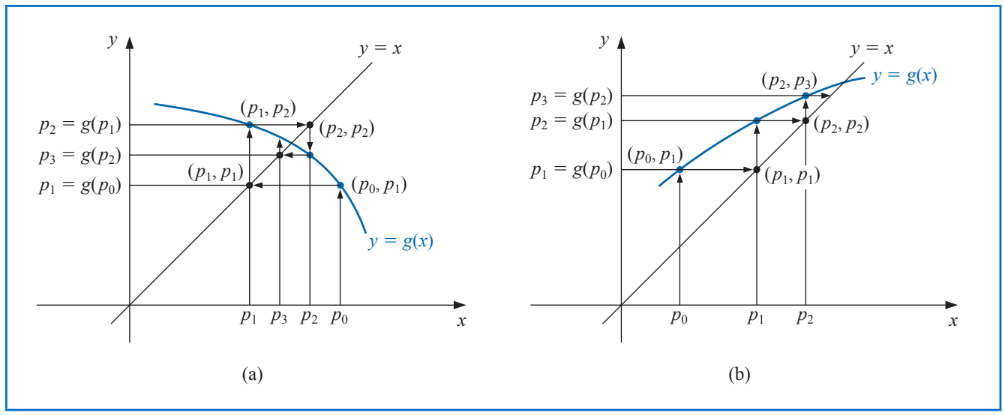
\includegraphics[width=0.8\linewidth]{figures/fixed_point_iteration_placeholder.png}
\caption{Minh họa quá trình lặp điểm cố định: (a) hội tụ chậm, (b) hội tụ nhanh.}
\label{fig:fixed_point_iteration}
\end{figure}

%-------------------------------------------------------------
\begin{algorithm}[!h]
\caption{Fixed-Point Iteration}
\label{alg:fixed_point_iteration}
\begin{algorithmic}[1]
\State Chọn xấp xỉ ban đầu $p_0$; ngưỡng sai số $\text{TOL}$; số lặp tối đa $N_0$.
\State $i \gets 1$.
\While{$i \le N_0$}
    \State $p \gets g(p_0)$ \hfill \% tính giá trị lặp mới
    \If{$|p - p_0| < \text{TOL}$}
        \State \Return $p$ \hfill \% thuật toán thành công
    \EndIf
    \State $i \gets i + 1$
    \State $p_0 \gets p$ \hfill \% cập nhật giá trị lặp
\EndWhile
\State \Return \texttt{"Thất bại: vượt quá $N_0$ vòng lặp."}
\end{algorithmic}
\end{algorithm}


%-------------------------------------------------------------
\subsubsection*{Ví dụ minh họa}

Xét phương trình
\[
x^3 + 4x^2 - 10 = 0,
\]
phương trình này có nghiệm duy nhất trong $[1,2]$ (xem lại Ví dụ~\ref{subsec:example1}).

Ta có thể viết lại phương trình về dạng điểm cố định $x = g(x)$ theo nhiều cách.
Ví dụ:
\begin{align*}
\text{(a)}\;& x = g_1(x) = x - x^3 - 4x^2 + 10,\\
\text{(b)}\;& x = g_2(x) = \sqrt{10/x - 4x},\\
\text{(c)}\;& x = g_3(x) = \tfrac{1}{2}\sqrt{10 - x^3},\\
\text{(d)}\;& x = g_4(x) = \sqrt{\tfrac{10}{4 + x}},\\
\text{(e)}\;& x = g_5(x) = x - \frac{x^3 + 4x^2 - 10}{3x^2 + 8x}.
\end{align*}

Giả sử chọn $p_0 = 1.5$, ta thực hiện thuật toán~\ref{alg:fixed_point_iteration} cho mỗi hàm $g_i$.

\begin{table}[!h]
\centering
\caption{Kết quả của phương pháp lặp điểm cố định cho năm dạng $g_i$.}
\label{tab:fixed_point_results}
\begin{tabular}{c|ccccc}
\toprule
$n$ & (a) & (b) & (c) & (d) & (e) \\
\midrule
0  & 1.5 & 1.5 & 1.5 & 1.5 & 1.5 \\
1  & -0.875 & 0.8165 & 1.28695 & 1.34840 & 1.37333 \\
2  & 6.732 & 2.9969 & 1.40254 & 1.36737 & 1.36521 \\
3  & -469.7 & $\sqrt{-8.65}$ & 1.34546 & 1.36496 & 1.36523 \\
4  & $1.03\times10^8$ & --- & 1.37517 & 1.36526 & 1.36523 \\
5  & --- & --- & 1.36009 & 1.36522 & 1.36523 \\
10 & --- & --- & 1.36478 & 1.36523 & 1.36523 \\
15 & --- & --- & 1.36522 & 1.36523 & 1.36523 \\
20 & --- & --- & 1.36523 & 1.36523 & 1.36523 \\
25 & --- & --- & 1.36523 & 1.36523 & 1.36523 \\
30 & --- & --- & 1.36523 & 1.36523 & 1.36523 \\
\bottomrule
\end{tabular}
\end{table}

Nghiệm thật (so sánh từ Ví dụ~\ref{subsec:example1}) là:
\[
p = 1.365230013.
\]
Ta thấy các lựa chọn (c), (d), và (e) hội tụ nhanh đến nghiệm thật, trong khi (a) phân kỳ
và (b) trở nên không xác định (do biểu thức căn của số âm).

\begin{remark}
Phương pháp chia đôi yêu cầu 27 vòng lặp để đạt cùng độ chính xác $10^{-4}$,
trong khi các biến thể điểm cố định như (c)–(e) chỉ cần chưa đến 10 vòng lặp.
Điều này minh họa sức mạnh của việc chọn dạng $g(x)$ thích hợp.
\end{remark}

\begin{theorem}[Định lý điểm cố định]
\label{thm:fixed_point_theorem}
Giả sử $g \in C[a,b]$ và $g(x)\in[a,b]$ với mọi $x\in[a,b]$.  
Giả sử thêm rằng $g'(x)$ tồn tại trên $(a,b)$ và tồn tại hằng số $k$ với $0<k<1$ sao cho
\[
|g'(x)| \le k, \qquad \forall x \in (a,b).
\]
Khi đó, với mọi giá trị khởi tạo $p_0 \in [a,b]$, dãy được xác định bởi
\[
p_n = g(p_{n-1}), \qquad n \ge 1,
\]
hội tụ đến điểm cố định duy nhất $p \in [a,b]$ của $g$.
\end{theorem}

\begin{proof}
Theo Định lý~\ref{thm:fixed_point_existence_uniqueness}, $g$ có đúng một điểm cố định $p$ sao cho $g(p)=p$.  
Với mỗi $n\ge1$, áp dụng Định lý Giá trị Trung bình (Mean Value Theorem) cho $g$ trên khoảng $(p_{n-1},p)$, tồn tại $\xi_n \in (a,b)$ sao cho
\[
|p_n - p|
  = |g(p_{n-1}) - g(p)|
  = |g'(\xi_n)|\,|p_{n-1}-p|
  \le k\,|p_{n-1}-p|.
\]
Suy ra theo quy nạp
\[
|p_n - p| \le k^n |p_0 - p|.
\tag{*}\label{eq:fixedpoint_error}
\]
Vì $0<k<1$, ta có $\lim_{n\to\infty} k^n = 0$, do đó
\[
\lim_{n\to\infty} |p_n - p| = 0,
\]
nghĩa là $\{p_n\}$ hội tụ đến $p$.
\end{proof}

\begin{corollary}[Sai số của phép lặp điểm cố định]
\label{cor:fixed_point_error}
Nếu $g$ thỏa các giả thiết của Định lý~\ref{thm:fixed_point_theorem}, thì sai số khi dùng $p_n$ để xấp xỉ $p$ được chặn bởi
\begin{align}
|p_n - p| &\le k^n \max\{|p_0 - a|,\;|b - p_0|\}, \label{eq:fixedpoint_bound1}\\[3pt]
|p_n - p| &\le \frac{k^n}{1-k}\,|p_1 - p_0|, \qquad n \ge 1. \label{eq:fixedpoint_bound2}
\end{align}
\end{corollary}

\begin{proof}
Vì $p\in[a,b]$, từ bất đẳng thức~\eqref{eq:fixedpoint_error} suy ra
\[
|p_n - p| \le k^n |p_0 - p| \le k^n \max\{|p_0 - a|,\,|b - p_0|\},
\]
cho~\eqref{eq:fixedpoint_bound1}.  

Tiếp theo, theo chứng minh của Định lý~\ref{thm:fixed_point_theorem},
\[
|p_{n+1} - p_n| = |g(p_n) - g(p_{n-1})|
 \le k\,|p_n - p_{n-1}|.
\]
Suy ra bằng quy nạp
\[
|p_{n+j} - p_{n+j-1}| \le k^{j-1}|p_1 - p_0|.
\]
Tổng các sai số vi phân này cho $m>n\ge1$:
\[
|p_m - p_n|
  \le \sum_{i=n}^{m-1}|p_{i+1}-p_i|
  \le |p_1 - p_0|\!\!\sum_{i=n}^{m-1}\!k^i
  \le \frac{k^n}{1-k}|p_1 - p_0|.
\]
Cho $m\!\to\!\infty$ ta được~\eqref{eq:fixedpoint_bound2}.
\end{proof}

\subsubsection*{Phân tích các hàm lặp điểm cố định}

Xét lại các hàm $g_1, g_2, g_3, g_4, g_5$ được sử dụng trong ví dụ trước, theo định lý điểm cố định~\ref{thm:fixed_point_theorem} và hệ quả~\ref{cor:fixed_point_error}.

\paragraph*{(a) Hàm $g_1(x) = x - x^3 - 4x^2 + 10$}

Ta có $g_1(1) = 6$ và $g_1(2) = -12$, do đó $g_1$ không ánh xạ đoạn $[1,2]$ vào chính nó.  
Thêm nữa, $g_1'(x) = 1 - 3x^2 - 8x$, nên $|g_1'(x)| > 1$ với mọi $x \in [1,2]$.  
Theo định lý điểm cố định, điều kiện này không đảm bảo hội tụ — vì vậy không có lý do để mong đợi phương pháp này hội tụ.

\paragraph*{(b) Hàm $g_2(x) = \sqrt{10/x - 4x}$}

Với $x \in [1,2]$, ta thấy $g_2$ không ánh xạ $[1,2]$ vào chính nó, và dãy $\{p_n\}$ không xác định tại $p_0 = 1.5$.  
Hơn nữa, khoảng chứa nghiệm $p \approx 1.365$ cho ta $|g_2'(x)| \approx 3.4 > 1$, do đó không có cơ sở để kỳ vọng hội tụ.

\paragraph*{(c) Hàm $g_3(x) = \tfrac{1}{2}\sqrt{10 - x^3}$}

Ta có:
\[
g_3'(x) = -\frac{3}{4}x^2 (10 - x^3)^{-1/2} < 0 \quad \text{trên } [1,2],
\]
nên $g_3$ là hàm giảm nghiêm ngặt.  
Tuy nhiên $|g_3'(x)| \ge 2.12$ trên $[1,2]$, nên điều kiện $|g'(x)| \le k < 1$ không được thỏa mãn.  
Quan sát dãy $\{p_n\}$ với $p_0 = 1.5$ cho thấy chỉ cần xét trên đoạn $[1.15, 1.5]$ — tại đây $|g_3'(x)| < 1$, và vì $g_3$ giảm nghiêm ngặt, ta có:
\[
1.28 \approx g_3(1.5) \le g_3(x) \le g_3(1.1) = 1.5,
\]
nên dãy hội tụ đến nghiệm.

\paragraph*{(d) Hàm $g_4(x) = \sqrt{\tfrac{10}{4+x}}$}

Đạo hàm:
\[
|g_4'(x)| = \frac{5}{\sqrt{10(4+x)^3}} \le \frac{5}{\sqrt{10(4+1)^3}} < 0.15, \quad \forall x \in [1,2].
\]
Vì $|g_4'(x)| < 1$, theo định lý điểm cố định, dãy $\{p_n\}$ hội tụ nhanh đến nghiệm thật.

\paragraph*{(e) Hàm $g_5(x) = x - \frac{x^3 + 4x^2 - 10}{3x^2 + 8x}$}

Hàm này được xây dựng sao cho đạo hàm tại nghiệm gần như bằng 0, và quả thật:
\[
|g_5'(x)| \text{ nhỏ hơn nhiều so với } |g_3'(x)|.
\]
Điều này giải thích tại sao $g_5$ cho tốc độ hội tụ nhanh hơn đáng kể.

\medskip
Từ những kết quả trên, ta có thể rút ra:

\begin{itemize}
\item Làm thế nào để tìm một hàm $g$ sao cho dãy $\{p_n\}$ hội tụ đáng tin cậy và nhanh chóng đến nghiệm của bài toán $f(x)=0$?
\item \textbf{Trả lời:} Biến đổi bài toán tìm nghiệm $f(x)=0$ thành bài toán điểm cố định $x=g(x)$ sao cho $|g'(x)|$ nhỏ nhất có thể gần nghiệm $p$.
\end{itemize}

%-------------------------------------------------------------
\paragraph*{Triển khai trên Maple}

Trong phần mềm Maple, gói NumericalAnalysis có sẵn lệnh FixedPointIteration.  
Ví dụ sau minh họa việc sử dụng:

\begin{verbatim}
> with(Student[NumericalAnalysis]):

> g := x -> x - (x^3 + 4*x^2 - 10)/(3*x^2 + 8*x);
> FixedPointIteration(fixedpointiterator = g, x = 1.5,
                      tolerance = 1e-8, output = sequence,
                      maxiterations = 20);
\end{verbatim}

Maple trả về:
\[
1.5,\; 1.3733333,\; 1.365262015,\; 1.365230014,\; 1.365230013.
\]

Ta thấy kết quả hội tụ rất nhanh đến nghiệm chính xác $p = 1.365230013$,
xác nhận tính hiệu quả của lựa chọn hàm $g_5(x)$.


\section{Phương pháp Newton và các mở rộng}
Phương pháp Newton, hay còn gọi là phương pháp Newton-Raphson, là một trong những phương pháp giải bài toán tìm nghiệm (root-finding) nổi tiếng và mạnh mẽ nhất trong phân tích số.

\subsection{Phương pháp Newton}

Có nhiều cách để giới thiệu về phương pháp Newton.

Nếu chỉ quan tâm đến thuật toán, chúng ta có thể tiếp cận phương pháp Newton một cách trực quan, tức là xem xét kỹ thuật này dựa trên đồ thị. Ở cách tiếp cận này, phương pháp Newton được minh họa bằng việc sử dụng tiếp tuyến của đồ thị hàm số tại một điểm gần nghiệm để xấp xỉ nghiệm của phương trình.

Một cách tiếp cận khác là xây dựng phương pháp Newton như một kỹ thuật nhằm đạt được tốc độ hội tụ nhanh hơn so với các loại phương pháp lặp hàm khác. Phương pháp Newton nổi bật bởi khả năng hội tụ rất nhanh đến nghiệm thực sự khi điểm khởi đầu đủ gần nghiệm, nhanh hơn nhiều so với các phương pháp lặp điểm cố định thông thường (fixed-point iteration).

Cách thứ ba để giới thiệu về phương pháp Newton là dựa trên đa thức Taylor. Khi sử dụng khai triển Taylor để xây dựng phương pháp Newton, chúng ta không chỉ thu được công thức lặp đặc trưng của phương pháp, mà còn xác định được một giới hạn sai số (error bound) cho nghiệm gần đúng sau mỗi bước lặp. Điều này rất quan trọng trong thực tế, vì nó cho phép đánh giá mức độ chính xác của nghiệm thu được, đồng thời cung cấp cơ sở toán học vững chắc cho việc sử dụng phương pháp Newton trong các bài toán giải tích số.
\subsubsection*{Cơ sở lý thuyết}

{Giả sử rằng $f \in C^2[a, b]$.} Cho $p_0 \in [a, b]$ là một giá trị xấp xỉ cho nghiệm $p$ sao cho $f'(p_0) \neq 0$ và $|p - p_0|$ là nhỏ. Xét khai triển Taylor cấp một của $f(x)$ quanh $p_0$ và đánh giá tại $x = p$:

$$f(p) = f(p_0) + (p - p_0) f'(p_0) + \frac{(p - p_0)^2}{2} f''(\xi(p))$$
trong đó $\xi(p)$ nằm giữa $p$ và $p_0$. Do $f(p) = 0$, phương trình này trở thành:
$$0 = f(p_0) + (p - p_0) f'(p_0) + \frac{(p - p_0)^2}{2} f''(\xi(p))$$

Phương pháp Newton được xây dựng bằng cách giả sử rằng vì $|p - p_0|$ nhỏ, nên thành phần chứa $(p - p_0)^2$ là rất nhỏ và có thể bỏ qua, tức là:

$$0 \approx f(p_0) + (p - p_0) f'(p_0)$$

Giải phương trình này theo $p$ ta được:

$$p \approx p_0 - \frac{f(p_0)}{f'(p_0)}$$

Điều này thiết lập nền tảng cho phương pháp Newton, bắt đầu với giá trị xấp xỉ ban đầu $p_0$ và tạo ra dãy lặp $\{p_n\}$ theo công thức:

$$p_n = p_{n-1} - \frac{f(p_{n-1})}{f'(p_{n-1})},\quad n \geq 1.$$

\begin{figure}[H]
    \centering
    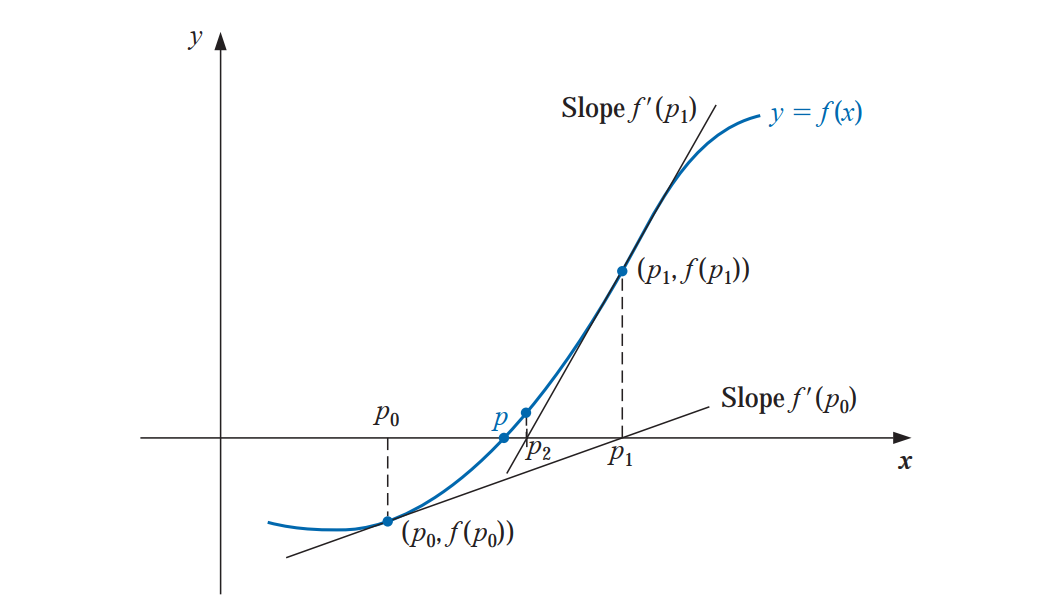
\includegraphics[width=1\linewidth]{figures/newton method.png}
    \caption{Minh họa hình học của phương pháp Newton}
    \label{fig:placeholder}
\end{figure}

Hình~\ref{fig:placeholder} minh họa cách các giá trị xấp xỉ được xác định thông qua các tiếp tuyến liên tiếp. 
Bắt đầu từ giá trị xấp xỉ ban đầu $p_0$, giá trị xấp xỉ kế tiếp $p_1$ được xác định là hoành độ của giao điểm giữa trục hoành và tiếp tuyến của đồ thị hàm $f$ tại điểm $(p_0, f(p_0))$. Tương tự, giá trị xấp xỉ $p_2$ là hoành độ của giao điểm giữa trục hoành và tiếp tuyến của đồ thị $f$ tại điểm $(p_1, f(p_1))$, và quá trình này tiếp tục như vậy. 

\subsubsection*{Thuật toán}

\begin{algorithm}[H]
\caption{Phương pháp Newton}
\label{alg:newton}
\begin{algorithm}[!h]
\SetAlgoLined
\KwIn{
    Hàm $f(x)$, đạo hàm $f'(x)$;\\
    Giá trị ban đầu $p_0$;\\
    Sai số cho phép $\mathrm{TOL}$;\\
    Số lần lặp tối đa $N_0$.
}
\KwOut{
    Nghiệm xấp xỉ $p$ hoặc thông báo lỗi nếu phương pháp thất bại.
}
\BlankLine
\caption{Thuật toán Newton–Raphson}
\label{alg:newton_method}
\end{algorithm}


\BlankLine
\textbf{Bước 1.} Đặt $i = 1$. \\
\textbf{Bước 2.} \While{$i \leq N_0$}{
    Tính $p = p_0 - \dfrac{f(p_0)}{f'(p_0)}$. \\
    \If{$|p - p_0| < \text{TOL}$}{
        Xuất $p$ (nghiệm xấp xỉ) và \textbf{dừng}.}
    Cập nhật $p_0 = p$. \\
    Tăng $i = i + 1$.
}
\textbf{Bước 3.} Nếu $i > N_0$, xuất thông báo: “Phương pháp thất bại sau $N_0$ lần lặp.”
\end{algorithm}

\subsubsection*{Điều kiện dừng}

Trong quá trình lặp của phương pháp Newton, ta cần xác định tiêu chí dừng thích hợp 
để kết luận rằng nghiệm xấp xỉ $p_n$ đã đủ gần với nghiệm thực $p$ của phương trình $f(x)=0$. 
Thông thường, một trong ba điều kiện sau được sử dụng:

\begin{enumerate}
    \item \textbf{Sai số tuyệt đối nhỏ:}
    \[
        |p_{n} - p_{n-1}| < \varepsilon,
    \]
    với $\varepsilon$ là sai số cho phép (tolerance). 
    Điều kiện này đảm bảo hai lần lặp liên tiếp cho kết quả gần nhau.

    \item \textbf{Sai số tương đối nhỏ:}
    \[
        \frac{|p_{n} - p_{n-1}|}{|p_{n}|} < \varepsilon.
    \]
    Điều kiện này thường được dùng khi giá trị nghiệm có thể lớn hoặc nhỏ, 
    giúp kiểm soát mức độ chính xác tương đối.

    \item \textbf{Giá trị hàm gần bằng 0:}
    \[
        |f(p_n)| < \varepsilon.
    \]
    Điều kiện này đảm bảo rằng $p_n$ gần với nghiệm thực của $f(x)=0$ về mặt giá trị hàm.
\end{enumerate}

\subsubsection*{Đặc điểm hội tụ của phương pháp Newton}

Giả sử $f \in C^2[a,b]$, $p$ là nghiệm thực của phương trình $f(x) = 0$, 
và $f'(p) \neq 0$. Khi đó, nếu giá trị khởi tạo $p_0$ được chọn đủ gần với $p$, 
dãy $\{p_n\}$ được xác định bởi công thức lặp
\[
    p_{n} = p_{n-1} - \frac{f(p_{n-1})}{f'(p_{n-1})},
\]
sẽ \textbf{hội tụ bậc hai} (quadratic convergence) về nghiệm $p$.

Điều này có nghĩa là tồn tại một hằng số $C > 0$ sao cho
\[
    |p_{n+1} - p| \leq C\,|p_n - p|^2.
\]
Nói cách khác, \emph{sai số của lần lặp tiếp theo tỉ lệ với bình phương sai số của lần lặp trước đó}. 
Do đó, khi dãy $\{p_n\}$ tiến gần nghiệm, số chữ số chính xác trong nghiệm xấp xỉ gần như tăng gấp đôi sau mỗi bước lặp.

\begin{center}
\textit{Tốc độ hội tụ bậc hai là ưu điểm nổi bật nhất của phương pháp Newton.}
\end{center}

Tuy nhiên, phương pháp này chỉ đảm bảo hội tụ nhanh khi các điều kiện sau được thỏa mãn:
\begin{enumerate}
    \item Hàm $f(x)$ khả vi liên tục và $f'(x)$ không triệt tiêu trong lân cận của nghiệm $p$.
    \item Giá trị ban đầu $p_0$ được chọn đủ gần nghiệm thực $p$.
    \item Đạo hàm $f'(x)$ có thể được tính chính xác hoặc xấp xỉ tốt.
\end{enumerate}

Nếu các điều kiện trên không được thỏa mãn, phương pháp Newton có thể:
\begin{itemize}
    \item hội tụ chậm hoặc phân kỳ (diverge),
    \item dao động giữa các giá trị (oscillate),
    \item hoặc hội tụ về một nghiệm khác không mong muốn.
\end{itemize}

\noindent
Ví dụ, nếu $f'(p_0) = 0$, công thức lặp sẽ không xác định do mẫu số bằng không. Vì vậy, trong thực hành tính toán, việc chọn giá trị ban đầu $p_0$ hợp lý và kiểm tra đạo hàm $f'(x)$ là bước rất quan trọng trước khi áp dụng phương pháp Newton.

\newtheorem{theorem}{Định lý}
\begin{theorem}
Giả sử $f \in C^2[a, b]$. 
Nếu tồn tại $p \in (a, b)$ sao cho $f(p) = 0$ và $f'(p) \neq 0$, 
thì tồn tại $\delta > 0$ sao cho phương pháp Newton sinh ra dãy 
$\{p_n\}_{n=1}^{\infty}$ hội tụ về $p$ với mọi giá trị khởi tạo 
$p_0 \in [p - \delta,\, p + \delta]$.
\end{theorem}

\subsubsection*{Ví dụ minh họa}

Xét phương trình
\[
    f(x) = \cos x - x = 0.
\]
Ta sẽ sử dụng phương pháp Newton để tìm nghiệm xấp xỉ của phương trình này.

\textbf{Bước 1. Xác định đạo hàm.}
\[
    f'(x) = -\sin x - 1.
\]

\textbf{Bước 2. Chọn giá trị khởi tạo.}
Chọn $p_0 = \frac{\pi}{4} \approx 0.785398$.

\textbf{Bước 3. Áp dụng công thức Newton.}
\[
    p_{n} = p_{n-1} - \frac{f(p_{n-1})}{f'(p_{n-1})} 
           = p_{n-1} - \frac{\cos(p_{n-1}) - p_{n-1}}{-\sin(p_{n-1}) - 1}.
\]

\textbf{Bước 4. Thực hiện các bước lặp.}
Ta thu được các giá trị sau:

\begin{center}
\begin{tabular}{|c|c|}
\hline
\textbf{Lần lặp} $n$ & \textbf{Giá trị xấp xỉ} $p_n$ \\
\hline
0 & 0.7853981635 \\
1 & 0.7395361337 \\
2 & 0.7390851781 \\
3 & 0.7390851332 \\
\hline
\end{tabular}
\end{center}

\textbf{Kết quả.}
Sau ba lần lặp, dãy $\{p_n\}$ hội tụ đến nghiệm
\[
    p \approx 0.7390851332,
\]
chính là nghiệm của phương trình $x = \cos x$.

\subsubsection*{Ví dụ minh họa}
\begin{itemize}
    \item Sai số giảm rất nhanh sau mỗi lần lặp, phản ánh tính \textbf{hội tụ bậc hai} của phương pháp Newton.
    \item Nếu chọn giá trị ban đầu $p_0$ nằm xa nghiệm thật, quá trình có thể phân kỳ hoặc dao động.
    \item Trong thực hành, có thể dừng khi $|p_{n} - p_{n-1}| < 10^{-6}$ hoặc $|f(p_n)| < 10^{-6}$.
\end{itemize}

\subsection{Các mở rộng của phương pháp Newton}
\subsubsection{Phương pháp Secant}
Phương pháp Secant là một mở rộng của phương pháp Newton, 
nhằm khắc phục nhược điểm cần tính đạo hàm $f'(x)$ tại mỗi bước lặp. 
Thay vì tính đạo hàm chính xác, phương pháp này sử dụng \textbf{sai phân hữu hạn} để xấp xỉ đạo hàm.

\paragraph*{Ý tưởng.}
Xuất phát từ công thức Newton:
\[
    p_{n} = p_{n-1} - \frac{f(p_{n-1})}{f'(p_{n-1})},
\]
thay đạo hàm $f'(p_{n-1})$ bằng sai phân:
\[
    f'(p_{n-1}) \approx 
    \frac{f(p_{n-1}) - f(p_{n-2})}{p_{n-1} - p_{n-2}}.
\]
Khi đó, công thức lặp trở thành:
\[
    p_{n} = p_{n-1} - f(p_{n-1})
    \frac{p_{n-1} - p_{n-2}}{f(p_{n-1}) - f(p_{n-2})}.
\]

\begin{figure}[H]
    \centering
    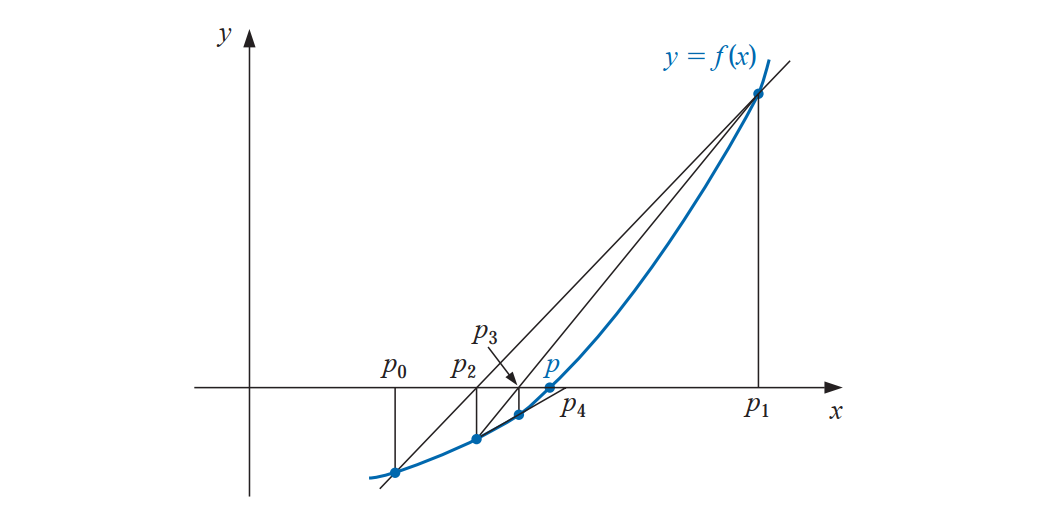
\includegraphics[width=1\linewidth]{figures/secant.png}
    \caption{Minh họa hình học của phương pháp Secant}
    \label{fig:placeholder}
\end{figure}

Bắt đầu với hai giá trị xấp xỉ ban đầu $p_0$ và $p_1$, 
giá trị xấp xỉ $p_2$ được xác định là \textbf{hoành độ của giao điểm giữa trục hoành và đường thẳng nối hai điểm} $(p_0, f(p_0))$ và $(p_1, f(p_1))$ trên đồ thị hàm $f$. Tương tự, giá trị xấp xỉ $p_3$ là hoành độ của giao điểm giữa trục hoành và đường thẳng nối hai điểm $(p_1, f(p_1))$ và $(p_2, f(p_2))$, và quá trình này tiếp tục như vậy.
Lưu ý rằng kể từ khi $p_2$ được xác định, mỗi bước của phương pháp Secant \textbf{chỉ cần một lần tính giá trị hàm $f(x)$}. 
Ngược lại, mỗi bước của phương pháp Newton yêu cầu đánh giá cả 
\textbf{hàm $f(x)$ và đạo hàm $f'(x)$}.

\paragraph*{Thuật toán Secant.}
\begin{enumerate}
    \item Chọn hai giá trị khởi tạo $p_0$ và $p_1$, cùng sai số cho phép $\text{TOL}$ và số lần lặp tối đa $N_0$.
    \item Với $i = 2, 3, \ldots, N_0$:
    \begin{enumerate}
        \item Tính
        \[
            p_i = p_{i-1} - f(p_{i-1})
            \frac{p_{i-1} - p_{i-2}}{f(p_{i-1}) - f(p_{i-2})}.
        \]
        \item Nếu $|p_i - p_{i-1}| < \text{TOL}$ hoặc $|f(p_i)| < \text{TOL}$, dừng và xuất $p_i$.
        \item Ngược lại, gán $p_{i-2} = p_{i-1}$ và $p_{i-1} = p_i$ rồi tiếp tục.
    \end{enumerate}
    \item Nếu vượt quá $N_0$ lần lặp, thông báo “Phương pháp thất bại”.
\end{enumerate}

\paragraph*{Đặc điểm.}
\begin{itemize}
    \item Không cần tính đạo hàm $f'(x)$.
    \item Cần hai giá trị khởi tạo $p_0$ và $p_1$.
    \item Tốc độ hội tụ \textbf{siêu tuyến tính} với bậc khoảng $1.618$ (bằng số vàng).
    \item Có thể phân kỳ nếu $p_0$ và $p_1$ không đủ gần nghiệm thật.
\end{itemize}

\paragraph*{Ví dụ minh họa.}
Giải phương trình $f(x) = \cos x - x = 0$ bằng phương pháp Secant 
với $p_0 = 0.5$, $p_1 = 0.785398$.

\begin{center}
\begin{tabular}{|c|c|}
\hline
\textbf{Lần lặp} $n$ & \textbf{Giá trị xấp xỉ} $p_n$ \\
\hline
0 & 0.5000000000 \\
1 & 0.7853980000 \\
2 & 0.7362990000 \\
3 & 0.7391190000 \\
4 & 0.7390851000 \\
\hline
\end{tabular}
\end{center}

Sau vài lần lặp, ta được $p \approx 0.7390851$, 
rất gần với nghiệm thật của phương trình $x = \cos x$.

\paragraph*{Nhận xét.}
Phương pháp Secant thường được ưa dùng khi:
\begin{itemize}
    \item đạo hàm của $f(x)$ khó hoặc tốn kém để tính toán;
    \item hoặc ta chỉ có giá trị hàm tại các điểm đã biết.
\end{itemize}
Tuy tốc độ hội tụ của phương pháp Secant chậm hơn Newton (bậc $\approx 1.618 < 2$), nhưng ưu điểm là \textbf{không cần đạo hàm}, giúp nó linh hoạt và hiệu quả hơn trong nhiều bài toán thực tế.

\subsubsection*{Phương pháp False Position}

Phương pháp \textit{False Position} hay còn gọi là \textit{Regula Falsi} 
là một biến thể của phương pháp Secant. 
Tương tự Secant, nó dùng đường thẳng đi qua hai điểm trên đồ thị hàm $f(x)$ 
để xấp xỉ nghiệm của phương trình $f(x) = 0$, 
nhưng có điểm khác biệt quan trọng là \textbf{đảm bảo nghiệm luôn nằm trong đoạn ban đầu}.

\paragraph*{Ý tưởng.}
Giả sử ta có hai điểm ban đầu $a$ và $b$ sao cho
\[
    f(a) \cdot f(b) < 0,
\]
tức là $f(x)$ đổi dấu trên đoạn $[a, b]$ và do đó tồn tại ít nhất một nghiệm $p \in (a, b)$ 
theo định lý giá trị trung gian.  
Phương pháp False Position xác định nghiệm xấp xỉ đầu tiên bằng công thức Secant:
\[
    p = b - f(b)\frac{b - a}{f(b) - f(a)}.
\]
Nếu $f(a)f(p) < 0$, ta thay $b = p$; ngược lại, nếu $f(b)f(p) < 0$, ta thay $a = p$.  
Quá trình được lặp lại cho đến khi đạt sai số mong muốn.

\begin{figure}[H]
    \centering
    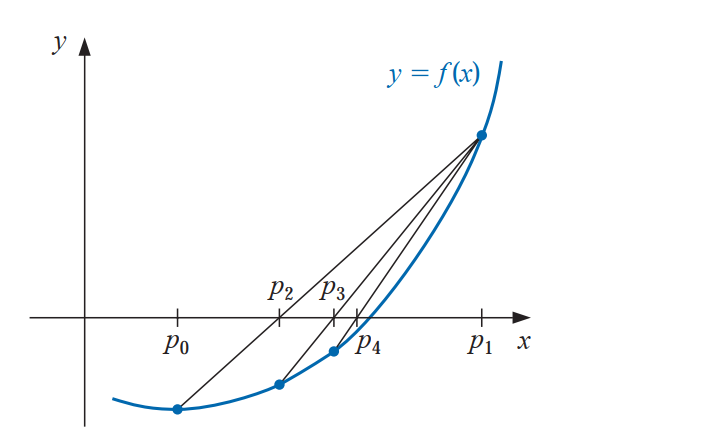
\includegraphics[width=1\linewidth]{figures/fasle position.png}
    \caption{Minh họa hình học của phương pháp False Position}
    \label{fig:placeholder}
\end{figure}


\paragraph*{Thuật toán False Position.}
\begin{enumerate}
    \item Cho hai giá trị $a$ và $b$ sao cho $f(a)f(b) < 0$.
    \item Tính $p$ bằng:
    \[
        p = b - f(b)\frac{b - a}{f(b) - f(a)}.
    \]
    \item Nếu $|f(p)| < \text{TOL}$ hoặc $|b - a| < \text{TOL}$, dừng và xuất $p$.
    \item Nếu $f(a)f(p) < 0$, gán $b = p$; ngược lại, gán $a = p$.
    \item Lặp lại các bước trên cho đến khi đạt điều kiện dừng.
\end{enumerate}

\paragraph*{Đặc điểm.}
\begin{itemize}
    \item Phương pháp False Position luôn \textbf{duy trì đoạn chứa nghiệm}, 
    nên đảm bảo hội tụ (giống phương pháp chia đôi).
    \item Tuy nhiên, tốc độ hội tụ chỉ là \textbf{tuyến tính}, 
    chậm hơn phương pháp Newton và Secant.
    \item Nếu $f(x)$ có độ dốc lớn ở một đầu đoạn, các giá trị $a$ hoặc $b$ có thể bị “cố định”, 
    làm quá trình hội tụ rất chậm.
\end{itemize}

\paragraph*{Ví dụ minh họa.}
Giải phương trình $f(x) = \cos x - x = 0$ bằng phương pháp False Position 
với đoạn ban đầu $[a, b] = [0, 1]$.

\begin{center}
\begin{tabular}{|c|c|c|c|}
\hline
\textbf{Lần lặp} $n$ & $a_n$ & $b_n$ & $p_n$ \\
\hline
0 & 0.000000 & 1.000000 & 0.685074 \\
1 & 0.685074 & 1.000000 & 0.736299 \\
2 & 0.736299 & 1.000000 & 0.739119 \\
3 & 0.739119 & 1.000000 & 0.739085 \\
\hline
\end{tabular}
\end{center}

Kết quả thu được sau vài bước lặp là 
\[
    p \approx 0.739085,
\]
trùng với nghiệm thật của phương trình $x = \cos x$.

\paragraph*{Nhận xét.}
\begin{itemize}
    \item Phương pháp False Position kết hợp ưu điểm của phương pháp chia đôi (đảm bảo hội tụ) và phương pháp Secant (hội tụ nhanh hơn).
    \item Dù vậy, trong thực tế, nếu cần hội tụ nhanh hơn, người ta thường dùng \textbf{phương pháp Secant} hoặc \textbf{Newton}.
\end{itemize}

\section{Phân tích sai số trong các phương pháp lặp}

\subsection{Bậc hội tụ (Order of Convergence)}
\subsubsection*{Định nghĩa bậc hội tụ}

Giả sử $\{p_n\}$ là dãy các giá trị xấp xỉ hội tụ đến nghiệm thực $p$ của một phương trình $f(x) = 0$, và đặt sai số tại bước $n$ là 
\[
e_n = p_n - p.
\]
Dãy $\{p_n\}$ được gọi là \textbf{hội tụ đến $p$ với bậc hội tụ $\alpha > 0$} nếu tồn tại một hằng số $\lambda \ge 0$ sao cho
\[
    \lim_{n \to \infty} 
    \frac{|p_{n+1} - p|}{|p_n - p|^{\alpha}} = \lambda.
\]

Khi đó:
\begin{itemize}
    \item $\alpha$ được gọi là \textbf{bậc hội tụ (order of convergence)};
    \item $\lambda$ được gọi là \textbf{hằng số hội tụ (rate constant)}.
\end{itemize}

\paragraph*{Các trường hợp đặc biệt:}
\begin{enumerate}
    \item Nếu $\alpha = 1$ và $0 < \lambda < 1$, dãy có \textbf{hội tụ tuyến tính}:
    \[
        |e_{n+1}| \approx \lambda |e_n|
    \]
    \item Nếu $\alpha = 2$, dãy có \textbf{hội tụ bậc hai}:
    \[
        |e_{n+1}| \approx \lambda |e_n|^2
    \]

\end{enumerate}

\paragraph*{Nhận xét:}
\begin{itemize}
    \item Bậc hội tụ càng cao thì phương pháp càng nhanh đạt đến nghiệm thật.
    \item Tuy nhiên, phương pháp có bậc hội tụ cao thường yêu cầu nhiều phép tính hơn mỗi bước 

\end{itemize}

\begin{theorem}
Giả sử $g \in C[a, b]$ và thỏa mãn $g(x) \in [a, b]$ với mọi $x \in [a, b]$. 
Giả sử thêm rằng $g$ khả vi trên $(a, b)$ và tồn tại một hằng số dương $k < 1$ sao cho
\[
    |g'(x)| \le k, \quad \forall x \in (a, b).
\]
Nếu $g'(p) \ne 0$, thì với mọi giá trị khởi tạo $p_0 \ne p$ trong $[a, b]$, 
dãy $\{p_n\}$ được xác định bởi
\[
    p_n = g(p_{n-1}), \quad n \ge 1,
\]
hội tụ \textbf{tuyến tính} đến \textbf{điểm cố định duy nhất} $p \in [a, b]$.
\end{theorem}

Trường hợp đặc biệt khi $g'(p) = 0$ dẫn đến tốc độ hội tụ nhanh hơn. 
Kết quả sau đây chỉ ra rằng khi đó, dãy lặp sẽ hội tụ ít nhất với bậc hai.

\begin{theorem}
Giả sử $p$ là nghiệm của phương trình $x = g(x)$. 
Giả sử thêm rằng $g'(p) = 0$ và $g$ khả vi liên tục trên một khoảng mở $I$ chứa $p$, với $|g''(x)| < M$ trên $I$ cho một hằng số dương $M$.

Khi đó tồn tại $\delta > 0$ sao cho với mọi giá trị khởi tạo 
$p_0 \in [p - \delta,\, p + \delta]$, dãy lặp
\[
    p_n = g(p_{n-1}), \quad n \ge 1,
\]
hội tụ \textbf{ít nhất bậc hai} đến $p$. Hơn nữa, với $n$ đủ lớn, ta có ước lượng sai số:
\[
    |p_{n+1} - p| < \frac{M}{2}\, |p_n - p|^2.
\]
\end{theorem}

\paragraph*{Hàm lặp và điều kiện hội tụ bậc hai}
Hai định lý trên cho thấy rằng, để một phương pháp lặp dạng cố định đạt được tốc độ hội tụ bậc hai, 
ta cần xây dựng hàm lặp $g(x)$ sao cho:
\[
    g(p) = p \quad \text{và} \quad g'(p) = 0.
\]
Một cách tự nhiên để xây dựng hàm như vậy từ phương trình $f(x) = 0$
là cộng hoặc trừ một bội số của $f(x)$ vào $x$. 
Xét dãy lặp dạng
\[
    p_n = g(p_{n-1}), \quad n \ge 1,
\]
với
\[
    g(x) = x - \phi(x) f(x),
\]
trong đó $\phi(x)$ là một hàm khả vi sẽ được xác định sao cho quá trình lặp hội tụ nhanh.
Tính đạo hàm của $g(x)$:
\[
    g'(x) = 1 - \phi'(x)f(x) - \phi(x)f'(x).
\]
Tại nghiệm $p$ của $f(x) = 0$, ta có $f(p) = 0$, nên:
\[
    g'(p) = 1 - \phi(p)f'(p).
\]
Để đạt được hội tụ bậc hai, ta cần $g'(p) = 0$, do đó:
\[
    \phi(p) = \frac{1}{f'(p)}.
\]
Nếu ta chọn $\phi(x) = 1 / f'(x)$, thì điều kiện trên được thỏa mãn, và phương pháp lặp thu được chính là:
\[
    p_n = p_{n-1} - \frac{f(p_{n-1})}{f'(p_{n-1})},
\]
tức là \textbf{phương pháp Newton (Newton's Method)}.\\

Từ đó suy ra rằng, nếu $f(p) = 0$ và $f'(p) \ne 0$, 
thì với điểm khởi tạo $p_0$ đủ gần nghiệm thật $p$, 
phương pháp Newton hội tụ ít nhất với \textbf{bậc hai}. 
Điều này giải thích vì sao Newton’s Method 
là một trong những phương pháp tìm nghiệm nhanh và hiệu quả nhất trong thực hành.

\captionsetup[table]{skip=10pt}
\begin{table}[H]
\centering
\caption{\textit{Bảng so sánh bậc hội tụ của các phương pháp lặp phổ biến}}
\label{tab:order_of_convergence}
\begin{adjustbox}{max width=\textwidth}
\begin{tabular}{|l|l|c|l|}
\hline
\textbf{Phương pháp} & \textbf{Công thức lặp} & \textbf{Bậc hội tụ $\alpha$} & \textbf{Đặc điểm nổi bật} \\ \hline
Bisection 
& $p_{n} = \dfrac{a_n + b_n}{2}$ 
& $1.0$ (tuyến tính) 
& Luôn hội tụ, nhưng chậm. \\ \hline

Fixed-Point 
& $p_n = g(p_{n-1})$ 
& $1.0$ 
& Dễ cài đặt, phụ thuộc vào $|g'(p)| < 1$. \\ \hline

Secant 
& $p_n = p_{n-1} - f(p_{n-1}) 
\dfrac{p_{n-1} - p_{n-2}}{f(p_{n-1}) - f(p_{n-2})}$ 
& $\approx 1.618$ 
& Không cần đạo hàm, hội tụ nhanh. \\ \hline

Newton 
& $p_n = p_{n-1} - \dfrac{f(p_{n-1})}{f'(p_{n-1})}$ 
& $2.0$ 
& Rất nhanh, cần đạo hàm. \\ \hline

Modified Newton 
& $p_n = p_{n-1} - 
\dfrac{f(p_{n-1}) f'(p_{n-1})}
{[f'(p_{n-1})]^2 - f(p_{n-1}) f''(p_{n-1})}$ 
& $3.0$ 
& Cần đạo hàm bậc hai, hội tụ cực nhanh. \\ \hline
\end{tabular}
\end{adjustbox}
\end{table}

\paragraph*{Kết luận.}
Bậc hội tụ là thước đo tốc độ tiệm cận nghiệm của các phương pháp lặp. 
Nó cho biết mức độ giảm sai số qua từng bước tính toán.

\subsection{Nghiệm bội (Multiple Roots)}

\paragraph*{Định nghĩa.}
Giả sử $f(x)$ là một hàm khả vi nhiều lần trên khoảng $I$, và $p$ là nghiệm của phương trình $f(x) = 0$. 
Khi đó, $p$ được gọi là \textbf{nghiệm bội $m$} (root of multiplicity $m$) của $f$ 
nếu:
\[
    f(p) = 0, \quad f'(p) = 0, \quad f''(p) = 0, \quad \dots, \quad f^{(m-1)}(p) = 0,
\]
nhưng
\[
    f^{(m)}(p) \ne 0.
\]
Nói cách khác, $p$ là nghiệm của $f(x)$ và đồng thời là nghiệm của tất cả các đạo hàm bậc nhỏ hơn $m$, nhưng không phải là nghiệm của đạo hàm bậc $m$.

\paragraph*{Ví dụ.}
\begin{itemize}
    \item Hàm $f(x) = (x - 2)^2$ có nghiệm bội $m = 2$ tại $p = 2$.
    \item Hàm $f(x) = (x - 1)^3$ có nghiệm bội $m = 3$ tại $p = 1$.
\end{itemize}

\paragraph*{Giải thích hình học.}
Nếu $p$ là nghiệm bội lớn hơn $1$, đồ thị của $f(x)$ 
\textbf{chạm} trục hoành tại $x = p$ nhưng không cắt qua nó.  
Ví dụ, với $f(x) = (x - 2)^2$, 
đồ thị tiếp xúc với trục hoành tại $x=2$ thay vì cắt qua, do đó Newton’s Method sẽ hội tụ chậm hơn trong vùng lân cận điểm này.
\\
Để mô tả rõ hơn hành vi này, các định lý sau đây trình bày chi tiết tốc độ hội tụ của phương pháp Newton cổ điển, phương pháp Newton cải tiến cho nghiệm bội, và phương pháp Secant.

% --- THEOREM 2.10 ---
\begin{theorem}
Giả sử $f \in C^{2}[a,b]$ và $p \in (a,b)$ là nghiệm bội $m$ của $f$, tức là
\[
    f(p) = f'(p) = \dots = f^{(m-1)}(p) = 0, \quad f^{(m)}(p) \ne 0.
\]
Nếu $p_0$ đủ gần $p$, thì dãy được xác định bởi công thức Newton
\[
    p_{n+1} = p_n - \frac{f(p_n)}{f'(p_n)}, \quad n \ge 0,
\]
hội tụ đến $p$ với \textbf{tốc độ tuyến tính} và hằng số hội tụ xấp xỉ
\[
    |p_{n+1} - p| \approx \frac{m-1}{m}\,|p_n - p|.
\]
\end{theorem}

\begin{theorem}
Giả sử $f \in C^{2}[a,b]$ và $p \in (a,b)$ là nghiệm bội $m$ của $f$. 
Khi đó, phương pháp Newton cải tiến
\[
    p_{n+1} = p_n - \frac{m\, f(p_n)}{f'(p_n)}, \quad n \ge 0,
\]
hội tụ đến $p$ với \textbf{bậc hội tụ hai} đối với mọi giá trị khởi tạo $p_0$ đủ gần $p$.
\end{theorem}

\begin{theorem}
Giả sử $f \in C^{2}[a,b]$ và $p$ là nghiệm đơn của $f$. 
Khi đó, phương pháp Secant 
\[
    p_{n} = p_{n-1} - f(p_{n-1}) \cdot 
    \frac{p_{n-1} - p_{n-2}}{f(p_{n-1}) - f(p_{n-2})}, \quad n \ge 2,
\]
hội tụ đến $p$ với \textbf{bậc hội tụ} xấp xỉ $\alpha \approx 1.618$, 
tức là tốc độ hội tụ \textbf{siêu tuyến tính (superlinear)}.
\end{theorem}

\paragraph*{Nhận xét:}
\begin{itemize}
    \item \textbf{Định lý~4} cho thấy khi nghiệm có bội số $m > 1$, 
    phương pháp Newton tiêu chuẩn chỉ hội tụ tuyến tính với hằng số hội tụ $\tfrac{m-1}{m}$.  
    Điều này giải thích hiện tượng hội tụ chậm khi đồ thị của $f(x)$ 
    tiếp xúc với trục hoành tại nghiệm (thay vì cắt qua).

    \item \textbf{Định lý~5} khắc phục hạn chế này bằng cách 
    nhân thêm hệ số $m$ trong công thức Newton.  
    Hệ số này hiệu chỉnh lại độ dốc tiếp tuyến và 
    khôi phục \textbf{tốc độ hội tụ bậc hai} như trong trường hợp nghiệm đơn.

    \item \textbf{Định lý~6} mô tả một phương pháp thay thế – 
    \textbf{phương pháp Secant} – 
    không yêu cầu đạo hàm, nhưng vẫn đạt tốc độ hội tụ nhanh 
    (bậc $\alpha \approx 1.618$).  
    Do đó, nó được xem là một sự cân bằng tốt giữa hiệu năng và chi phí tính toán.
\end{itemize}

\paragraph*{}
Ba định lý trên nhấn mạnh rằng:
\begin{itemize}
    \item Phương pháp Newton tiêu chuẩn có thể mất hiệu quả khi gặp nghiệm bội.
    \item Có thể khôi phục lại tốc độ hội tụ bậc hai 
    bằng cách sử dụng \textbf{phương pháp Newton cải tiến}.
    \item Trong các trường hợp không thể hoặc không muốn tính đạo hàm, 
    \textbf{phương pháp Secant} là lựa chọn hợp lý với tốc độ hội tụ siêu tuyến tính.
\end{itemize}
\subsubsection*{Ví dụ: Ảnh hưởng của nghiệm bội đến tốc độ hội tụ của Newton}

\paragraph*{}
Xét hàm
\[
    f(x) = e^x - x - 1.
\]
\begin{enumerate}
    \item Chứng minh rằng $f$ có nghiệm bội $2$ tại $x = 0$.
    \item Chứng minh rằng phương pháp Newton với $p_0 = 1$ hội tụ đến nghiệm này, 
    nhưng không hội tụ bậc hai.
\end{enumerate}

\paragraph*{(1) Chứng minh $x = 0$ là nghiệm bội $2$.}
Ta có
\[
    f(x) = e^x - x - 1, \quad f'(x) = e^x - 1, \quad f''(x) = e^x.
\]
Khi $x = 0$, ta được:
\[
    f(0) = 1 - 0 - 1 = 0, \quad f'(0) = 1 - 1 = 0, \quad f''(0) = 1 \ne 0.
\]
Do đó, $x = 0$ là \textbf{nghiệm bội $2$} của phương trình $f(x) = 0$.

\paragraph*{(2) Phân tích hội tụ của phương pháp Newton.}
Phương pháp Newton có công thức lặp:
\[
    p_{n+1} = p_n - \frac{f(p_n)}{f'(p_n)}.
\]
Thay $f(x) = e^x - x - 1$ và $f'(x) = e^x - 1$ vào ta được:
\[
    p_{n+1} = p_n - \frac{e^{p_n} - p_n - 1}{e^{p_n} - 1}.
\]

\paragraph*{Tính gần nghiệm $x = 0$.}
Khai triển $e^x$ quanh $x=0$:
\[
    e^x = 1 + x + \frac{x^2}{2} + O(x^3).
\]
Khi đó:
\[
    f(x) = \frac{x^2}{2} + O(x^3), \quad f'(x) = x + \frac{x^2}{2} + O(x^3).
\]
Suy ra:
\[
    \frac{f(x)}{f'(x)} 
    = \frac{\tfrac{x^2}{2} + O(x^3)}{x + \tfrac{x^2}{2} + O(x^3)} 
    = \frac{x}{2} + O(x^2).
\]
Do đó, phép lặp Newton gần nghiệm có dạng:
\[
    p_{n+1} = p_n - \frac{f(p_n)}{f'(p_n)} = p_n - \left( \frac{p_n}{2} + O(p_n^2) \right)
    = \frac{p_n}{2} + O(p_n^2).
\]
Bỏ qua thành phần bậc cao, ta có xấp xỉ:
\[
    |p_{n+1}| \approx \frac{1}{2} |p_n|.
\]

\paragraph*{Kết luận}
Sai số giảm xấp xỉ một nửa sau mỗi lần lặp, nghĩa là phương pháp Newton 
\textbf{hội tụ tuyến tính} với hằng số hội tụ $\lambda = \tfrac{1}{2}$, thay vì hội tụ bậc hai như trong trường hợp nghiệm đơn.

Nếu chọn $p_0 = 1$, ta có:
\[
\begin{array}{c|c}
n & p_n \\ \hline
0 & 1.000000 \\
1 & 0.53788284 \\
2 & 0.25577441 \\
3 & 0.12604745 \\
4 & 0.06285013 \\
5 & 0.03133119 \\
\end{array}
\]
Ta nhận thấy rằng $p_n \to 0$, nhưng giá trị giảm gần \emph{một nửa} sau mỗi bước, 
khớp với tốc độ hội tụ tuyến tính dự đoán ở trên.

\paragraph*{Nhận xét.}
Ví dụ này minh họa rằng:
\begin{itemize}
    \item Khi nghiệm là nghiệm bội, phương pháp Newton thông thường không còn hội tụ bậc hai.
    \item Trong trường hợp này ($m = 2$), tốc độ hội tụ chỉ còn tuyến tính với hệ số $\tfrac{1}{2}$.
    \item Nếu áp dụng \textbf{phương pháp Newton cải tiến}:
    \[
        p_{n+1} = p_n - \frac{2 f(p_n)}{f'(p_n)},
    \]
    thì hội tụ sẽ trở lại bậc hai như với nghiệm đơn.
\end{itemize}

\paragraph*{Nhận xét.}
\begin{itemize}
    \item Sai số giảm rất nhanh sau mỗi vòng lặp, 
    chứng tỏ phương pháp Newton có hiệu quả vượt trội 
    khi giá trị khởi tạo đủ gần nghiệm thật.
    \item Bậc hội tụ thực nghiệm $\alpha \approx 2$ khớp với 
    kết quả lý thuyết trong phần “Order of Convergence”.
    \item Nếu nghiệm là nghiệm bội, tốc độ hội tụ sẽ giảm 
    xuống tuyến tính như đã nêu trong Định lý~4.
\end{itemize}

\section{Tăng tốc hội tụ (Accelerating Convergence)}

Trong các phần trước, ta đã xem xét các phương pháp lặp 
và phân tích tốc độ hội tụ của chúng thông qua khái niệm \textit{bậc hội tụ}.
Ta đã thấy rằng các phương pháp như Newton’s Method có thể đạt \textbf{bậc hội tụ hai},
trong khi nhiều phương pháp khác – chẳng hạn như \textit{phương pháp cố định điểm} 
hoặc \textit{phương pháp dây cung} – chỉ đạt được \textbf{hội tụ tuyến tính} hoặc 
\textbf{siêu tuyến tính}.

Mặc dù các phương pháp hội tụ tuyến tính có ưu điểm là dễ tính toán,
nhưng chúng thường cần rất nhiều bước lặp để đạt được độ chính xác mong muốn.
Điều này làm tăng đáng kể chi phí tính toán khi áp dụng trong thực tế.
Vì vậy, một hướng tiếp cận tự nhiên là tìm cách \textbf{tăng tốc quá trình hội tụ}
mà không phải thay đổi bản chất của phương pháp lặp ban đầu.
Phần này giới thiệu hai kỹ thuật phổ biến được sử dụng cho mục đích đó:
\textbf{Aitken’s $\Delta^2$ Process} và \textbf{Steffensen’s Method}.
Hai phương pháp này có thể biến một dãy hội tụ tuyến tính thành một dãy hội tụ nhanh hơn, thậm chí đạt tới bậc hai trong nhiều trường hợp.

\subsection{Aitken’s $\Delta^2$ Process}

\paragraph*{Ý tưởng.}
Giả sử $\{p_n\}$ là một dãy hội tụ tuyến tính đến $p$, tức là tồn tại hằng số $0 < \lambda < 1$ sao cho
\[
    p_{n+1} - p \approx \lambda (p_n - p).
\]
Trong trường hợp như vậy, hội tụ thường diễn ra khá chậm.  
Mục tiêu của \textbf{phép biến đổi Aitken’s $\Delta^2$} 
là tạo ra một dãy mới $\{\hat{p}_n\}$ hội tụ nhanh hơn đến cùng giới hạn $p$.

\paragraph*{Công thức biến đổi.}
Gọi sai phân bậc nhất và bậc hai của dãy $\{p_n\}$ lần lượt là:
\[
    \Delta p_n = p_{n+1} - p_n, \qquad
    \Delta^2 p_n = \Delta p_{n+1} - \Delta p_n = p_{n+2} - 2p_{n+1} + p_n.
\]
Phép biến đổi Aitken định nghĩa dãy mới:
\[
    \hat{p}_n = p_n - \frac{(\Delta p_n)^2}{\Delta^2 p_n}
    = p_n - \frac{(p_{n+1} - p_n)^2}{p_{n+2} - 2p_{n+1} + p_n}.
\]
Nếu $\{p_n\}$ hội tụ tuyến tính, thì $\{\hat{p}_n\}$ thường hội tụ nhanh hơn đáng kể, 
thậm chí \textbf{siêu tuyến tính} trong nhiều trường hợp.

\paragraph*{Giải thích trực giác.}
Phép biến đổi này dựa trên việc \emph{nội suy tuyến tính} 
ba giá trị liên tiếp $p_n, p_{n+1}, p_{n+2}$ 
để ước lượng trực tiếp giới hạn $p$.  
Thay vì chờ dãy $\{p_n\}$ dần tiến tới $p$, 
Aitken’s process sử dụng dạng sai phân để dự đoán trước điểm hội tụ.

\paragraph*{Ví dụ minh họa.}
Xét dãy hội tụ tuyến tính:
\[
    p_n = 1 + \frac{1}{2^n}, \quad n = 0,1,2,\dots
\]
Rõ ràng $p = 1$.  
Ta tính:
\[
    p_0 = 1.5, \quad p_1 = 1.25, \quad p_2 = 1.125.
\]
Khi đó:
\[
    \Delta p_0 = p_1 - p_0 = -0.25, \quad
    \Delta^2 p_0 = p_2 - 2p_1 + p_0 = 0.125.
\]
Áp dụng công thức Aitken:
\[
    \hat{p}_0 = p_0 - \frac{(\Delta p_0)^2}{\Delta^2 p_0}
               = 1.5 - \frac{(-0.25)^2}{0.125} = 1.5 - 0.5 = 1.0.
\]
Chỉ sau một bước, ta đã thu được chính xác nghiệm $p = 1$, 
trong khi dãy gốc cần vô hạn bước để đạt tới giới hạn đó.  
Điều này cho thấy sức mạnh của Aitken’s $\Delta^2$ process 
trong việc tăng tốc hội tụ.

\paragraph*{Lưu ý.}
\begin{itemize}
    \item Phép biến đổi Aitken chỉ áp dụng hiệu quả khi dãy $\{p_n\}$ 
    hội tụ tuyến tính và $\Delta^2 p_n \ne 0$.
    \item Nếu dãy gốc đã hội tụ siêu tuyến tính hoặc bậc hai, 
    việc áp dụng Aitken có thể không cải thiện đáng kể (hoặc làm nhiễu kết quả do sai số làm tròn).
\end{itemize}

\paragraph*{Kết luận.}
Phương pháp Aitken’s $\Delta^2$ là một công cụ đơn giản nhưng hiệu quả 
để cải thiện tốc độ hội tụ của các dãy tuyến tính.  

\subsection{Steffensen’s Method}

\paragraph*{Ý tưởng.}
Phương pháp của Steffensen được xây dựng bằng cách 
áp dụng \textbf{Aitken’s $\Delta^2$ Process} trực tiếp cho 
\textit{phương pháp lặp cố định điểm}:
\[
    p_{n+1} = g(p_n).
\]
Mục tiêu là cải thiện tốc độ hội tụ của quá trình lặp này, 
đặc biệt khi nó chỉ hội tụ tuyến tính.

\paragraph*{Cơ sở lý thuyết.}
Nếu ta gọi:
\[
    p_{n+1} = g(p_n), \qquad 
    p_{n+2} = g(p_{n+1}),
\]
thì theo công thức của Aitken, 
giá trị được tăng tốc bởi Steffensen là:
\[
    \hat{p}_n = p_n - 
    \frac{(p_{n+1} - p_n)^2}{p_{n+2} - 2p_{n+1} + p_n}.
\]
Thay $p_{n+1} = g(p_n)$ và $p_{n+2} = g(g(p_n))$, 
ta thu được công thức của \textbf{Steffensen’s Method}:
\[
    p_{n+1} = p_n - 
    \frac{[g(p_n) - p_n]^2}{g(g(p_n)) - 2g(p_n) + p_n}.
\]
Phương pháp này không yêu cầu đạo hàm của $f(x)$, 
nhưng trong nhiều trường hợp vẫn đạt tốc độ hội tụ bậc hai.

\paragraph*{Liên hệ với Newton’s Method.}
Nếu ta chọn
\[
    g(x) = x - \frac{f(x)}{f'(x)},
\]
thì Steffensen’s Method trở thành Newton’s Method.  
Do đó, Steffensen có thể xem là một cách 
\textbf{ước lượng đạo hàm} trong Newton bằng sai phân hữu hạn.

\paragraph*{Ví dụ minh họa.}
Xét phương trình
\[
    f(x) = e^{-x} - x = 0,
\]
với phương pháp lặp cố định điểm
\[
    g(x) = e^{-x}.
\]
Chọn giá trị khởi tạo $p_0 = 0$, ta có:
\[
\begin{aligned}
    g(p_0) &= e^{0} = 1, \\
    g(g(p_0)) &= e^{-1} \approx 0.3679.
\end{aligned}
\]
Áp dụng công thức Steffensen:
\[
    p_1 = p_0 - 
    \frac{[g(p_0) - p_0]^2}{g(g(p_0)) - 2g(p_0) + p_0}
        = 0 - \frac{(1 - 0)^2}{0.3679 - 2(1) + 0}
        \approx 0.6127.
\]
Tiếp tục lặp thêm vài bước, ta thu được:
\[
\begin{array}{c|c}
n & p_n \\ \hline
0 & 0.0000 \\
1 & 0.6127 \\
2 & 0.5666 \\
3 & 0.5671 \\
\end{array}
\]
Nghiệm đúng là $p = 0.567143$, 
và chỉ sau vài vòng lặp, phương pháp đã hội tụ rất nhanh 
mà không cần đạo hàm của $f$.

\paragraph*{Đặc điểm.}
\begin{itemize}
    \item Không yêu cầu đạo hàm $f'(x)$, chỉ cần giá trị của hàm $g(x)$.
    \item Hội tụ bậc hai nếu $g'(p) \ne 1$.
    \item Thích hợp cho các bài toán mà việc tính đạo hàm là phức tạp hoặc tốn kém.
\end{itemize}

\paragraph*{Kết luận.}
Phương pháp của Steffensen là một trong những kỹ thuật 
\textbf{tăng tốc hội tụ} quan trọng nhất trong giải tích số.
Nó kết hợp sự đơn giản của phương pháp lặp cố định điểm với tốc độ hội tụ của phương pháp Newton, mà không cần sử dụng đạo hàm.
\section{Tìm nghiệm của đa thức và phương pháp 
(MüllerZeros of Polynomials and Müller's Method)}

\subsection{Đa thức đại số (Algebraic Polynomials)}

Một đa thức đại số bậc $n$ được viết dưới dạng tổng quát:
\[
P(x) = a_nx^n + a_{n-1}x^{n-1} + \cdots + a_1x + a_0,
\]
trong đó $a_i$ là các hệ số thực hoặc phức, và $a_n \neq 0$.

Theo \textit{Định lý cơ bản của Đại số} (\textit{Fundamental Theorem of Algebra}), mỗi đa thức bậc $n$ có đúng $n$ nghiệm phức (tính cả bội).  
Nếu tất cả hệ số $a_i$ là số thực, thì các nghiệm phức xuất hiện theo cặp liên hợp phức.

Mục tiêu là tìm các nghiệm $r$ sao cho $P(r) = 0$. Trong thực tế, các nghiệm này thường được tìm gần đúng bằng các phương pháp số, vì nghiệm chính xác chỉ biểu diễn được tường minh khi đa thức có bậc nhỏ hơn hoặc bằng 4.

\subsection{Phương pháp Horner (Horner’s Method)}

Phương pháp Horner là một kỹ thuật hiệu quả để \textit{tính giá trị của đa thức} và thực hiện \textit{chia đa thức} cho $(x - x_0)$.  
Nó giúp giảm đáng kể số phép nhân và cộng cần thiết, đồng thời tăng độ ổn định số.

Cho đa thức:
\[
P(x) = a_nx^n + a_{n-1}x^{n-1} + \cdots + a_1x + a_0.
\]
Phương pháp Horner viết lại đa thức trên dưới dạng lồng nhau:
\[
P(x) = (\cdots((a_nx + a_{n-1})x + a_{n-2})x + \cdots + a_1)x + a_0.
\]

\textbf{Thuật toán Horner:}
\begin{enumerate}
    \item Đặt $b_n = a_n$.
    \item Tính lần lượt:
    \[
    b_k = a_k + x_0 b_{k+1}, \quad k = n-1, n-2, \ldots, 0.
    \]
    \item Khi đó $P(x_0) = b_0$.
\end{enumerate}

Nếu thực hiện phép chia đa thức $P(x)$ cho $(x - x_0)$, thì phần dư của phép chia chính là $P(x_0)$, còn các hệ số thương là $b_1, b_2, \ldots, b_n$.

\textbf{Ví dụ 1.}  
Tính $P(2)$ cho $P(x) = 2x^4 - 3x^3 + 4x^2 - x + 5$.

\[
\begin{array}{r|rrrrr}
x=2 & 2 & -3 & 4 & -1 & 5 \\ 
 &   & 4 & 2 & 12 & 22 \\ \hline
 & 2 & 1 & 6 & 11 & 27
\end{array}
\]
Kết quả $P(2) = 27$.  
Các hệ số $(2, 1, 6, 11)$ là hệ số của đa thức thương khi chia $P(x)$ cho $(x - 2)$.

\subsection{Nghiệm phức: Phương pháp Müller (Complex Zeros: Müller's Method)}

Phương pháp Müller là sự mở rộng của \textit{phương pháp Secant} (Secant Method).  
Thay vì dùng đường thẳng đi qua hai điểm để xấp xỉ hàm số, phương pháp Müller sử dụng \textbf{parabol} (đa thức bậc hai) đi qua ba điểm $(p_0, f(p_0))$, $(p_1, f(p_1))$, $(p_2, f(p_2))$ để ước lượng nghiệm của hàm.  
Điểm cắt của parabol này với trục hoành được dùng làm giá trị xấp xỉ mới $p_3$.  
Vì phương trình bậc hai có thể có nghiệm phức, nên phương pháp Müller có khả năng tìm được \textbf{nghiệm phức} của phương trình, ngay cả khi bắt đầu từ các giá trị thực.
\begin{figure}[H]
    \centering
    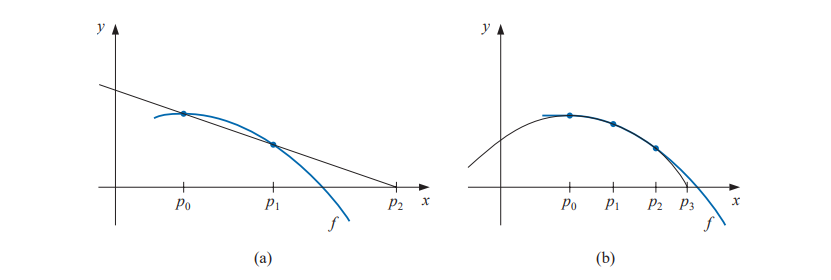
\includegraphics[width=1\linewidth]{figures/image.png}
    \caption{Minh họa hình học của phương pháp Müller}
    \label{fig:placeholder}
\end{figure}
\textbf{Ý tưởng.}  
Tại mỗi bước, ta tìm đa thức bậc hai nội suy $f(x)$ tại ba điểm gần nhau, rồi lấy giao điểm của parabol nội suy đó với trục $x$ làm điểm gần nghiệm kế tiếp.  
Công thức tổng quát của parabol nội suy có dạng:
\[
P(x) = a(x - p_2)^2 + b(x - p_2) + c,
\]
với $f_i = f(p_i)$.

Các hệ số $a,b,c$ được xác định bằng hiệu sai phân chia:
\[
\begin{aligned}
h_1 &= p_1 - p_0, \\
h_2 &= p_2 - p_1, \\
\delta_1 &= \frac{f_1 - f_0}{h_1}, \\
\delta_2 &= \frac{f_2 - f_1}{h_2}, \\
d &= \frac{\delta_2 - \delta_1}{h_2 + h_1}.
\end{aligned}
\]
Từ đó, ta có:
\[
a = d, \quad b = \delta_2 + h_2 d, \quad c = f_2.
\]

Giải phương trình $P(x) = 0$ cho ta nghiệm gần đúng mới:
\[
p_3 = p_2 - \frac{2c}{b \pm \sqrt{b^2 - 4ac}},
\]
trong đó dấu $\pm$ được chọn sao cho mẫu số có giá trị tuyệt đối lớn nhất (để tránh sai số trừ gần nhau):
\[
p_3 = p_2 - \frac{2c}{b + \operatorname{sgn}(b)\sqrt{b^2 - 4ac}}.
\]

Nếu $\Delta = b^2 - 4ac < 0$, phương pháp tự động sinh ra nghiệm phức, thể hiện khả năng xử lý nghiệm phức tự nhiên của nó.


\subsection{Thuật toán Müller (Müller’s Algorithm)}

\textbf{Các bước thực hiện:}
\begin{enumerate}
    \item Nhập $x_0, x_1, x_2$, sai số cho phép $TOL$, và số vòng lặp tối đa $N_0$.
    \item Với $i = 2, 3, \ldots, N_0$:
    \begin{align*}
        h_1 &= x_1 - x_0, & h_2 &= x_2 - x_1, \\
        \delta_1 &= \frac{f(x_1) - f(x_0)}{h_1}, & \delta_2 &= \frac{f(x_2) - f(x_1)}{h_2}, \\
        d &= \frac{\delta_2 - \delta_1}{h_2 + h_1}.
    \end{align*}
    Đặt $a = d$, $b = \delta_2 + h_2 d$, $c = f(x_2)$.
    \item Tính nghiệm gần đúng:
    \[
    x_3 = x_2 - \frac{2c}{b + \operatorname{sgn}(b)\sqrt{b^2 - 4ac}}.
    \]
    \item Nếu $|x_3 - x_2| < TOL$ hoặc $|f(x_3)| < TOL$, dừng lại.
    \item Ngược lại, đặt $x_0 = x_1, \; x_1 = x_2, \; x_2 = x_3$ và lặp lại.
\end{enumerate}

\textbf{Đặc điểm:}
\begin{itemize}
    \item Không cần đạo hàm của $f(x)$ như phương pháp Newton.
    \item Có thể tìm được nghiệm phức.
    \item Bậc hội tụ $\approx 1.84$ (nhanh hơn Secant, nhưng chậm hơn Newton).
    \item Cần ba giá trị khởi tạo ban đầu.
\end{itemize}

\textbf{Ví dụ 2.}  
Xét đa thức:
\[
f(x) = x^4 - 3x^3 + x^2 + x + 1.
\]
Chọn giá trị khởi tạo:
\[
x_0 = 0.5, \quad x_1 = -0.5, \quad x_2 = 0.
\]
Sau các bước lặp của phương pháp Müller, thu được:
\[
x_3 = -0.100000 + 0.888819i, \quad f(x_3) = -0.0112 + 3.0149i.
\]
Tiếp tục lặp, nghiệm hội tụ về:
\[
x \approx -0.339093 + 0.446630i.
\]
Do các hệ số của $f(x)$ là số thực, nên nghiệm liên hợp phức của nó cũng là nghiệm:
\[
\bar{x} = -0.339093 - 0.446630i.
\]
Nếu chọn các giá trị khởi tạo khác, chẳng hạn:
\[
x_0 = 1.5, \quad x_1 = 2.0, \quad x_2 = 2.5,
\]
thì phương pháp hội tụ đến nghiệm thực:
\[
x \approx 2.2888.
\]

\begin{figure}[H]
        \centering
        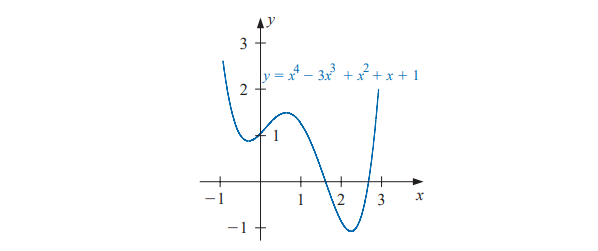
\includegraphics[width=1\linewidth]{figures/đt bậc 4.png}
        \caption{Đồ thị hàm số \[
f(x) = x^4 - 3x^3 + x^2 + x + 1.
\]}
    \label{fig:placeholder}
\end{figure}
        
\textbf{Nhận xét:}  
Phương pháp Müller có thể tìm được cả nghiệm thực và nghiệm phức của đa thức bậc cao, là một cải tiến đáng kể so với phương pháp Secant hoặc Newton khi xử lý các phương trình không có đạo hàm hoặc có nghiệm phức.

\textbf{Kết luận.}  
Phương pháp Müller là một sự mở rộng tự nhiên của phương pháp Secant, sử dụng nội suy bậc hai để xác định nghiệm gần đúng (có thể là phức) của phương trình phi tuyến.  
Với bậc hội tụ cao, không cần đạo hàm và khả năng phát hiện nghiệm phức, đây là công cụ mạnh trong việc tìm nghiệm của đa thức đại số bậc cao.  
Khi kết hợp với \textbf{kỹ thuật khử nghiệm (deflation)}, ta có thể lần lượt tìm được toàn bộ nghiệm của đa thức.


\section{Khử nghiệm của đa thức (Deflation of Polynomials)}

Sau khi tìm được một nghiệm của đa thức $P(x)$ (thực hoặc phức), ta thường muốn loại bỏ nghiệm đó để giảm bậc của đa thức và tiếp tục tìm các nghiệm còn lại.  
Quá trình loại bỏ nghiệm này được gọi là \textbf{deflation} (khử nghiệm hay khử bậc).

Giả sử $P(x)$ là đa thức bậc $n$ có dạng:
\[
P(x) = a_nx^n + a_{n-1}x^{n-1} + \cdots + a_1x + a_0,
\]
và ta đã tìm được nghiệm gần đúng $r$ của $P(x) = 0$. Khi đó, tồn tại một đa thức $Q(x)$ bậc $(n-1)$ sao cho:
\[
P(x) = (x - r)Q(x) + R,
\]
trong đó $R$ là phần dư. Nếu $r$ là nghiệm chính xác, thì $R = 0$.

\subsection{Khử nghiệm thực (Deflation for Real Roots)}

Để thực hiện phép chia này, ta sử dụng \textbf{phương pháp Horner} (Horner’s synthetic division).  
Ta viết:
\[
\begin{array}{r|rrrrr}
r & a_n & a_{n-1} & a_{n-2} & \cdots & a_0 \\ 
 &  & b_n & b_{n-1} & \cdots & b_1 \\ \hline
 & b_n & b_{n-1} & b_{n-2} & \cdots & b_0
\end{array}
\]
trong đó:
\[
\begin{aligned}
b_n &= a_n,\\
b_k &= a_k + r b_{k+1}, \quad k = n-1, n-2, \ldots, 0.
\end{aligned}
\]
Phần dư $R = b_0$, và các hệ số của đa thức thương $Q(x)$ là $b_n, b_{n-1}, \ldots, b_1$.  
Nếu $r$ chỉ là nghiệm gần đúng, ta có thể thực hiện \textit{một bước hiệu chỉnh} để cải thiện độ chính xác của $r$.

\textbf{Công thức hiệu chỉnh.}  
Giả sử sau khi khử nghiệm, ta được phần dư $R = P(r)$ và đa thức thương $Q(x)$.  
Theo Burden \& Faires, nghiệm $r$ có thể được hiệu chỉnh bằng công thức:
\[
r_{\text{new}} = r - \frac{R}{Q(r)}.
\]
Đây chính là \textit{một bước Newton} áp dụng cho hàm chia đa thức $(x - r)Q(x)$.

\textbf{Ví dụ 1.}  
Xét đa thức:
\[
P(x) = x^3 - 6x^2 + 11x - 6.
\]
Giả sử ta đã tìm được nghiệm $r = 1$.

Thực hiện Horner’s division:
\[
\begin{array}{r|rrrr}
1 & 1 & -6 & 11 & -6 \\ 
 &   & 1 & -5 & 6 \\ \hline
   & 1 & -5 & 6 & 0
\end{array}
\]
Đa thức thương là:
\[
Q(x) = x^2 - 5x + 6.
\]
Phần dư $R = 0$, chứng tỏ $x=1$ là nghiệm chính xác.  
Ta tiếp tục khử nghiệm trên $Q(x)$, ta được các nghiệm còn lại:
\[
x^2 - 5x + 6 = 0 \Rightarrow x = 2, 3.
\]

\subsection{Khử nghiệm phức (Deflation for Complex Roots)}

Khi nghiệm tìm được là \textbf{phức}, ví dụ $r = a + bi$ (với $b \ne 0$), thì nghiệm liên hợp $r^* = a - bi$ cũng là nghiệm (theo Định lý 2.20 trong sách):
\[
(x - r)(x - r^*) = x^2 - 2ax + (a^2 + b^2)
\]
là nhân tử bậc hai của $P(x)$.

Do đó, thay vì chia $P(x)$ cho $(x - r)$, ta thực hiện phép chia $P(x)$ cho \textbf{đa thức bậc hai thực}:
\[
x^2 - 2ax + (a^2 + b^2).
\]
Kết quả là một đa thức thực $Q(x)$ có bậc giảm 2, và phần dư $R(x)$ (nếu $r$ chỉ gần đúng) được dùng để hiệu chỉnh $a$ và $b$.

\textbf{Ví dụ 2.}  
Giả sử ta có đa thức:
\[
P(x) = x^4 - 3x^3 + x^2 + x + 1,
\]
và tìm được nghiệm gần đúng:
\[
r = -0.339093 + 0.446630i.
\]
Theo đó, nghiệm liên hợp là $r^* = -0.339093 - 0.446630i$.

Nhân tử bậc hai tương ứng:
\[
(x - r)(x - r^*) = x^2 - 2(-0.339093)x + [(-0.339093)^2 + (0.446630)^2] = x^2 + 0.678186x + 0.3125.
\]

Chia $P(x)$ cho nhân tử trên (dùng Horner mở rộng hoặc phép chia đa thức bậc hai) ta được:
\[
Q(x) = x^2 - 3.678186x + 3.200,
\]
với phần dư nhỏ (chứng tỏ nghiệm phức đã khá chính xác).

Giải $Q(x) = 0$ cho nghiệm thực còn lại:
\[
x = \frac{3.678186 \pm \sqrt{3.678186^2 - 4(3.200)}}{2} \Rightarrow x \approx 2.2888.
\]

\subsection{Phân tích và nhận xét}

\textbf{Đặc điểm.}
\begin{itemize}
    \item Deflation giúp giảm bậc của đa thức từng bước, nhờ đó dễ tìm các nghiệm còn lại.
    \item Với nghiệm thực, chỉ cần phép chia bậc 1 bằng Horner.
    \item Với nghiệm phức, cần chia bằng nhân tử bậc hai thực để tránh sai số phức không cần thiết.
    \item Khi nghiệm chỉ là gần đúng, việc deflation nhiều lần có thể tích luỹ sai số, vì vậy nên hiệu chỉnh lại nghiệm sau mỗi lần chia.
\end{itemize}

\textbf{Lưu ý quan trọng.}
\begin{itemize}
    \item Sau mỗi lần deflation, nên kiểm tra phần dư $R$ (hoặc $R(x)$) để đảm bảo nghiệm đủ chính xác.
    \item Nếu sai số còn lớn, áp dụng \textit{một hoặc vài bước Newton} trên đa thức gốc $P(x)$ để tinh chỉnh lại nghiệm.
    \item Khi tìm nghiệm phức, cần đảm bảo dùng biểu diễn số phức có độ chính xác kép để tránh làm tròn sai lệch giữa cặp liên hợp.
\end{itemize}

\textbf{Kết luận.}  
Phương pháp \textbf{deflation} là công cụ quan trọng giúp giảm bậc của đa thức sau khi tìm được một nghiệm (thực hoặc phức).  
Nó thường được sử dụng kết hợp với các thuật toán như \textbf{Müller’s Method} hoặc \textbf{Newton’s Method} để lần lượt xác định toàn bộ nghiệm của đa thức.  
Việc kiểm soát sai số và hiệu chỉnh nghiệm sau mỗi lần deflation là yếu tố then chốt đảm bảo độ chính xác của nghiệm cuối cùng.

% Chapter 2
\vspace*{1em}
\chapter{Các Phương Pháp Lặp Trong Đại Số Ma Trận}

\section{Các kỹ thuật lặp Jacobi và Gauss–Seide (The Jacobi and Gauss–Seidel Iterative Techniques)}

Trong phần này ta trình bày chi tiết hai phương pháp lặp cơ bản dùng để giải hệ tuyến tính
\[
A\mathbf{x}=\mathbf{b},\qquad A\in\mathbb{R}^{n\times n},\ \mathbf{b}\in\mathbb{R}^n,
\]
và sau đó đưa ra dạng tổng quát của các phương pháp lặp tuyến tính. Các phương pháp này là nền tảng
cho nhiều phương pháp lặp tiên tiến hơn (như SOR, CG, v.v.).

\subsection{Jacobi's Method}

\textbf{Phân rã ma trận.}
Ta phân rã ma trận $A$ theo
\[
A = D + L + U,
\]
trong đó $D$ là ma trận đường chéo gồm các $a_{ii}$, $L$ là ma trận tam giác dưới (phần dưới đường chéo, với dấu âm nếu muốn theo một dạng khác) và $U$ là ma trận tam giác trên, sao cho thường viết
\[
A = D - L - U
\]
khi muốn lấy $L$ và $U$ là các ma trận có dấu âm của các phần tử ngoài đường chéo.

\textbf{Dẫn xuất công thức Jacobi.}
Giải phương trình thứ $i$ trong $A\mathbf{x}=\mathbf{b}$ theo $x_i$:
\[
a_{ii} x_i = b_i - \sum_{\substack{j=1\\ j\ne i}}^{n} a_{ij} x_j,
\]
và do đó một công thức lặp thuần túy (không dùng phần tử vừa cập nhật) là
\[
x_i^{(k+1)} = \frac{1}{a_{ii}}\Big( b_i - \sum_{\substack{j=1\\ j\ne i}}^{n} a_{ij} x_j^{(k)}\Big),
\qquad i=1,\dots,n.
\]
Viết theo dạng vectơ, ta có dạng lặp
\[
\mathbf{x}^{(k+1)} = D^{-1}(\mathbf{b} - (L+U)\mathbf{x}^{(k)})
          = T_J \mathbf{x}^{(k)} + \mathbf{c}_J,
\]
với
\[
T_J = -D^{-1}(L+U),\qquad \mathbf{c}_J = D^{-1}\mathbf{b}.
\]

\textbf{Thuật toán Jacobi (tóm tắt).}
\begin{enumerate}
  \item Chọn một xấp xỉ khởi đầu $\mathbf{x}^{(0)}$.
  \item Với $k=0,1,2,\dots$ và với mỗi $i=1,\dots,n$ tính
    \[
    x_i^{(k+1)} = \frac{1}{a_{ii}}\Big( b_i - \sum_{j\ne i} a_{ij} x_j^{(k)}\Big).
    \]
  \item Dừng khi $\|\mathbf{x}^{(k+1)}-\mathbf{x}^{(k)}\|$ hoặc $\|A\mathbf{x}^{(k+1)}-\mathbf{b}\|$ nhỏ hơn một ngưỡng TOL.
\end{enumerate}

\textbf{Nhận xét về Jacobi.}
\begin{itemize}
  \item \textbf{Ưu điểm:} Rất dễ triển khai; mỗi bước cập nhật các thành phần độc lập dựa trên vòng trước → thuận lợi cho tính toán song song.
  \item \textbf{Nhược điểm:} Thường hội tụ chậm; cần điều kiện về cấu trúc ma trận để đảm bảo hội tụ.
\end{itemize}

\subsection{Jacobi Iterative — Điều kiện hội tụ}

\textbf{Ma trận lặp và spectral radius.}
Dạng tổng quát lặp tuyến tính là
\[
\mathbf{x}^{(k+1)} = T\mathbf{x}^{(k)} + \mathbf{c}.
\]
Một điều kiện cần và đủ để lặp hội tụ cho mọi xấp xỉ ban đầu là
\[
\rho(T) < 1,
\]
trong đó $\rho(T)$ là bán kính phổ của $T$ (max tuyệt đối các trị riêng).

\paragraph{Điều kiện đủ tiêu biểu.}
Một điều kiện dễ kiểm tra và thường dùng là \textbf{chéo trội nghiêm ngặt theo hàng}:
\[
|a_{ii}| > \sum_{j\ne i} |a_{ij}|,\qquad i=1,\dots,n.
\]
Nếu $A$ chéo trội theo hàng, thì cả ma trận Jacobi $T_J$ lẫn ma trận Gauss--Seidel $T_{GS}$ đều có $\rho<1$ và do đó hội tụ.

\textbf{Chuẩn và bất đẳng thức nghiệm.}
Dựa vào bất đẳng thức về chuẩn, nếu tồn tại một chuẩn ma trận $\|\cdot\|$ sao cho $\|T\|<1$ thì lặp hội tụ. Thực tế hay dùng chuẩn $\infty$ hoặc $1$ để kiểm tra chéo trội:
\[
\|T_J\|_\infty = \max_i \sum_{j\ne i} \frac{|a_{ij}|}{|a_{ii}|}.
\]

\subsection{The Gauss--Seidel Method}

\textbf{Ý tưởng.}
Gauss--Seidel tận dụng ngay các thành phần vừa được cập nhật trong cùng một vòng lặp để tính phần tử tiếp theo. Cách viết trực tiếp:
\[
x_i^{(k+1)} = \frac{1}{a_{ii}} \Big( b_i - \sum_{j=1}^{i-1} a_{ij} x_j^{(k+1)} - \sum_{j=i+1}^{n} a_{ij} x_j^{(k)}\Big),
\quad i=1,\dots,n.
\]

\textbf{Dạng ma trận lặp.}
Tách $A=D-L-U$ (chú ý dấu) thì
\[
(D-L)\mathbf{x}^{(k+1)} = U \mathbf{x}^{(k)} + \mathbf{b},
\]
và do đó
\[
\mathbf{x}^{(k+1)} = (D-L)^{-1} U \mathbf{x}^{(k)} + (D-L)^{-1}\mathbf{b},
\]
với ma trận lặp
\[
T_{GS} = (D-L)^{-1} U,\qquad \mathbf{c}_{GS} = (D-L)^{-1}\mathbf{b}.
\]

\textbf{Thuật toán Gauss--Seidel (tóm tắt).}
\begin{enumerate}
  \item Chọn xấp xỉ khởi đầu $\mathbf{x}^{(0)}$.
  \item Với $k=0,1,2,\dots$:
    \begin{itemize}
      \item Lần lượt cho $i=1,\dots,n$ tính
        \[
        x_i^{(k+1)} = \frac{1}{a_{ii}} \Big( b_i - \sum_{j=1}^{i-1} a_{ij} x_j^{(k+1)} - \sum_{j=i+1}^{n} a_{ij} x_j^{(k)}\Big).
        \]
    \end{itemize}
  \item Dừng khi đạt điều kiện dừng.
\end{enumerate}

\textbf{Nhận xét về Gauss--Seidel.}
\begin{itemize}
  \item \textbf{Ưu điểm:} Thường hội tụ nhanh hơn Jacobi; ít vòng lặp hơn để đạt độ chính xác tương đương.
  \item \textbf{Nhược điểm:} Khó song song hóa vì cập nhật tuần tự; mỗi vòng cần tính $(D-L)^{-1}u$ ẩn, nhưng thực tế thực hiện bằng công thức cập nhật trực tiếp nên không cần nghịch đảo rõ ràng.
\end{itemize}

\subsection{Gauss--Seidel Iterative — Điều kiện hội tụ}

\textbf{Các điều kiện tiêu biểu.}
\begin{itemize}
  \item Nếu $A$ là \textbf{chéo trội nghiêm ngặt theo hàng}, thì cả Jacobi và Gauss--Seidel hội tụ.
  \item Nếu $A$ là \textbf{đối xứng xác định dương} (SPD), Gauss--Seidel hội tụ (một phần có thể chứng minh dựa trên phân tích SPD và phương pháp năng lượng).
\end{itemize}

\textbf{So sánh ma trận lặp.}
Thường có quan hệ
\[
\rho(T_{GS}) \le \rho(T_J),
\]
vì Gauss--Seidel tận dụng nhiều thông tin hơn trong mỗi vòng lặp; do đó Gauss--Seidel thường hội tụ nhanh hơn (ít vòng hơn) so với Jacobi.

\subsection{General Iteration Methods (Dạng tổng quát của phương pháp lặp)}

\textbf{Tổng quát hóa.}
Một phương pháp lặp tuyến tính tổng quát có dạng
\[
\mathbf{x}^{(k+1)} = T\mathbf{x}^{(k)} + \mathbf{c},
\]
với $T$ được lựa chọn dựa trên phân rã $A=M-N$ sao cho
\[
M\mathbf{x}^{(k+1)} = N \mathbf{x}^{(k)} + \mathbf{b},
\]
và do đó
\[
\mathbf{x}^{(k+1)} = M^{-1}N \mathbf{x}^{(k)} + M^{-1}\mathbf{b},
\]
hay $T=M^{-1}N$. Các lựa chọn khác nhau của $M,N$ đưa ra các phương pháp khác nhau:
\begin{itemize}
  \item Jacobi: $M=D$, $N=-(L+U)$.
  \item Gauss--Seidel: $M=D-L$, $N=U$.
  \item SOR (sẽ trình bày ở 7.4): $M = \frac{1}{\omega}D - L$, $N = \frac{1-\omega}{\omega}D + U$.
\end{itemize}

\textbf{Tiêu chí chọn $M$.}
Muốn $M$ dễ giải (chẳng hạn tam giác hoặc đường chéo) để mỗi bước lặp rẻ chi phí, đồng thời $T=M^{-1}N$ có bán kính phổ nhỏ để hội tụ nhanh.

\textbf{Phân tích hội tụ.}
Để kiểm tra hội tụ, ta thường xét $\rho(T)$ hoặc một chuẩn ma trận $\|T\|$. Nếu $\rho(T)<1$ thì mọi xấp xỉ khởi đầu dẫn tới hội tụ; nếu $\rho(T)\ge1$ thì tối thiểu tồn tại xấp xỉ ban đầu khiến không hội tụ.

\textbf{Tốc độ hội tụ và lỗi.}
Nếu lặp hội tụ tuyến tính, tồn tại số $\mu\in(0,1)$ sao cho
\[
\|\mathbf{x}^{(k)}-\mathbf{x}\| \le C \mu^k
\]
với $\mu\approx\rho(T)$. Việc giảm $\rho(T)$ (qua chọn $M,N$ thích hợp hoặc qua tiền tiền xử lý/preconditioning) là mục tiêu chính của các phương pháp cải tiến.

\subsection{Ví dụ minh họa (cụ thể)}

\textbf{Hệ mẫu.} Xét hệ
\[
\begin{aligned}
10x_1 - x_2 + 2x_3 &= 6,\\
- x_1 + 11x_2 - x_3 + 3x_4 &= 25,\\
2x_1 - x_2 + 10x_3 - x_4 &= -11,\\
3x_2 - x_3 + 8x_4 &= 15.
\end{aligned}
\]
Ma trận là chéo trội nên cả Jacobi và Gauss--Seidel hội tụ.

\textbf{Jacobi (hai vòng lặp đầu).}
Với $\mathbf{x}^{(0)}=\mathbf{0}$,
\[
\begin{aligned}
x_1^{(1)} &= \tfrac{1}{10}(6 + 0 - 0) = 0.6,\\
x_2^{(1)} &= \tfrac{1}{11}(25 + 0 + 0 - 0) \approx 2.2727,\\
x_3^{(1)} &= \tfrac{1}{10}(-11 - 0 + 0 + 0) = -1.1,\\
x_4^{(1)} &= \tfrac{1}{8}(15 - 0 + 0) = 1.875.
\end{aligned}
\]
Dùng các giá trị này để tính vòng tiếp theo (mọi cập nhật dùng giá trị của vòng trước).

\textbf{Gauss--Seidel (hai vòng lặp đầu).}
Với $\mathbf{x}^{(0)}=\mathbf{0}$,
\[
\begin{aligned}
x_1^{(1)} &= 0.6,\\
x_2^{(1)} &= \tfrac{1}{11}(25 + x_1^{(1)} + 0 - 0) \approx \tfrac{1}{11}(25 + 0.6)=2.3273,\\
x_3^{(1)} &= \tfrac{1}{10}(-11 - 2x_1^{(1)} + x_2^{(1)} + 0)\approx -0.9575,\\
x_4^{(1)} &= \tfrac{1}{8}(15 - 3x_2^{(1)} + x_3^{(1)})\approx 1.8316.
\end{aligned}
\]
Ta thấy Gauss--Seidel sử dụng ngay $x_1^{(1)}$ khi tính $x_2^{(1)}$, do đó hội tụ nhanh hơn trong thực nghiệm.

\subsection{Kết luận}

\begin{itemize}
  \item \textbf{Jacobi} và \textbf{Gauss--Seidel} là hai phương pháp lặp cơ bản, dễ triển khai và phù hợp cho ma trận thưa.
  \item Kiểm tra hội tụ dựa trên \textbf{bán kính phổ} $\rho(T)$ hoặc điều kiện chéo trội.
  \item Dạng tổng quát $M\mathbf{x}^{(k+1)} = N\mathbf{x}^{(k)} + \mathbf{b}$ bao quát nhiều phương pháp; chọn $M$ sao cho dễ giải trong mỗi bước và làm giảm $\rho(M^{-1}N)$.
  \item Các phương pháp nâng cao (SOR, tiền xử lý, CG) phát triển trên nền tảng này để cải thiện tốc độ hội tụ và mở rộng vùng áp dụng.
\end{itemize}


\subsection*{Định nghĩa 7.23}
Giả sử \textbf(\( \tilde{x} \in \mathbb{R}^n \)) là một nghiệm xấp xỉ của \textbf{hệ phương trình tuyến tính} được xác định bởi Ax = b.
\textbf{Vectơ dư} (residual vector) của \( \tilde{x} \) đối với hệ này được định nghĩa là r = b - A\( \tilde{x} \). Khi \( \tilde{x} \) trùng với nghiệm chính xác của hệ, ta có \( r = 0 \).


\section{Các phương pháp lặp cải tiến trong giải hệ phương trình tuyến tính}

Chúng ta đã thấy trong Mục 7.3 rằng tốc độ hội tụ của một phương pháp lặp phụ thuộc vào bán kính phổ của ma trận liên quan đến phương pháp đó. Một cách để tăng tốc hội tụ là chọn phương pháp có ma trận với bán kính phổ nhỏ nhất. Trước khi trình bày quy trình chọn phương pháp như vậy, ta cần giới thiệu một cách đo mới cho biết mức độ sai khác giữa nghiệm xấp xỉ và nghiệm chính xác của hệ tuyến tính. Cách này sử dụng một vectơ được mô tả trong định nghĩa sau.

\subsection*{Định nghĩa 7.23}
Giả sử \textbf(\( \tilde{x} \in \mathbb{R}^n \)) là một nghiệm xấp xỉ của \textbf{hệ phương trình tuyến tính} được xác định bởi Ax = b.
\textbf{Vectơ dư} (residual vector) của \( \tilde{x} \) đối với hệ này được định nghĩa là r = b - A\( \tilde{x} \). Khi \( \tilde{x} \) trùng với nghiệm chính xác của hệ, ta có \( r = 0 \). Giả sử ta có:

\[
\mathbf{r}^{(k)} = \bigl(r^{(k)}_{1},\, r^{(k)}_{2},\, \ldots,\, r^{(k)}_{n}\bigr)^{t}.
\]

là \textbf{vectơ dư} của \textbf{phương pháp Gauss--Seidel}, tương ứng với \textbf{vectơ nghiệm xấp xỉ}

\[
\mathbf{x}^{(k)} = (x^{(k)}_1,\, x^{(k)}_2,\, \ldots,\, x^{(k)}_{i-1},\, x^{(k-1)}_i,\, \ldots,\, x^{(k-1)}_n)^{t}.
\]

Thành phần thứ \( m \) của vectơ \( r^{(k)} \) được cho bởi
\[
r^{(k)}_m = b_m - \sum_{j=1}^{i-1} a_{mj} x^{(k)}_j - \sum_{j=i}^{n} a_{mj} x^{(k-1)}_j, \tag{7.13}
\]
hay tương đương,
\[
r^{(k)}_m = b_m - \sum_{j=1}^{i-1} a_{mj} x^{(k)}_j - \sum_{j=i+1}^{n} a_{mj} x^{(k-1)}_j - a_{mi}x^{(k-1)}_i,
\]
với mỗi \( m = 1, 2, \ldots, n.\)

Đặc biệt, thành phần thứ \( i \) của \( r^{(k)} \) là
\[
r^{(k)}_i = b_i - \sum_{j=1}^{i-1} a_{ij}x^{(k)}_j - \sum_{j=i+1}^{n} a_{ij}x^{(k-1)}_j,
\]
do đó
\[
a_{ii}x^{(k-1)}_i + r^{(k)}_i = b_i - \sum_{j=1}^{i-1} a_{ij}x^{(k)}_j - \sum_{j=i+1}^{n} a_{ij}x^{(k-1)}_j. \tag{7.14}
\]

Nhắc lại rằng trong \textbf{phương pháp Gauss--Seidel}, \( x^{(k)}_i \) được chọn sao cho
\[
x^{(k)}_i = \frac{1}{a_{ii}}\left[b_i - \sum_{j=1}^{i-1} a_{ij}x^{(k)}_j - \sum_{j=i+1}^{n} a_{ij}x^{(k-1)}_j\right], \tag{7.15}
\]
vì vậy phương trình (7.14) có thể được viết lại thành
\[
a_{ii}x^{(k-1)}_i + r^{(k)}_i = a_{ii}x^{(k)}_i.
\]
Do đó, phương pháp Gauss--Seidel có thể được đặc trưng bởi điều kiện rằng \( x^{(k)}_i \) thỏa mãn
\[
x^{(k)}_i = x^{(k-1)}_i + \frac{r^{(k)}_i}{a_{ii}}. \tag{7.16}
\]

Ta có thể thiết lập thêm một mối liên hệ khác giữa các vectơ dư và kỹ thuật Gauss--Seidel. 
Xét vectơ dư \( r^{(k)}_{i+1} \) tương ứng với vectơ 
\(
x_{i+1}^{(k)} = (x^{(k)}_1,\, \ldots,\, x^{(k)}_i,\, x^{(k-1)}_{i+1},\, \ldots,\, x^{(k-1)}_n)^{t}.
\)
Theo công thức (7.13), thành phần thứ \( i+1 \) của \( r^{(k)} \) là
\[
r^{(k)}_{i+1} = b_{i+1} - \sum_{j=1}^{i} a_{i+1,j}x^{(k)}_j - \sum_{j=i+2}^{n} a_{i+1,j}x^{(k-1)}_j.
\]

Theo cách mà \( x_i^{(k)} \) được định nghĩa trong phương trình (7.15), ta thấy rằng \( r_{i+1}^{(k)} = 0 \). 
Theo nghĩa này, kỹ thuật Gauss--Seidel được đặc trưng bởi việc chọn mỗi \( x_{i+1}^{(k)} \) sao cho 
thành phần thứ \( i \) của vectơ dư \( r^{(k)} \) bằng không.

Tuy nhiên, việc chọn \( x_{i+1}^{(k)} \) sao cho một thành phần của vectơ dư bằng không 
không nhất thiết là cách hiệu quả nhất để giảm chuẩn của vectơ dư \( r_{i+1}^{(k)} \). 
Nếu ta sửa đổi quy trình Gauss--Seidel như trong phương trình (7.16), ta có

\[
x_i^{(k)} = x_i^{(k-1)} + \omega \frac{r_i^{(k)}}{a_{ii}}, \tag{7.17}
\]

thì với một số giá trị dương của \( \omega \), ta có thể giảm chuẩn của vectơ dư và 
đạt được tốc độ hội tụ nhanh hơn đáng kể.

Các phương pháp có chứa phương trình (7.17) được gọi là \textbf{phương pháp thư giãn} (relaxation methods).  
Với các giá trị \( \omega \) thỏa \( 0 < \omega < 1 \), các quy trình này được gọi là \textbf{phương pháp thư giãn dưới mức} (under-relaxation methods).  
Ta sẽ quan tâm đến các giá trị \( \omega \) lớn hơn 1, và các quy trình này được gọi là \textbf{phương pháp thư giãn quá mức} (over-relaxation methods).  
Chúng được sử dụng để tăng tốc độ hội tụ của các hệ mà phương pháp Gauss--Seidel có thể hội tụ.  
Các phương pháp này thường được viết tắt là \textbf{SOR} (Successive Over-Relaxation), 
và đặc biệt hữu ích trong việc giải các hệ tuyến tính phát sinh trong nghiệm số của các phương trình vi phân riêng phần.

Trước khi minh họa ưu điểm của phương pháp SOR, ta lưu ý rằng bằng cách sử dụng phương trình (7.14), 
ta có thể viết lại phương trình (7.17) dưới dạng thuận tiện cho việc tính toán như sau:

\[
x_i^{(k)} = (1 - \omega)x_i^{(k-1)} + \frac{\omega}{a_{ii}}
\left[
b_i - \sum_{j=1}^{i-1} a_{ij}x_j^{(k)} - \sum_{j=i+1}^{n} a_{ij}x_j^{(k-1)}
\right].
\]

Để xác định dạng ma trận của phương pháp SOR, ta viết lại biểu thức này như sau:

\[
a_{ii}x_i^{(k)} + \omega \sum_{j=1}^{i-1} a_{ij}x_j^{(k)} 
= (1 - \omega)a_{ii}x_i^{(k-1)} - \omega \sum_{j=i+1}^{n} a_{ij}x_j^{(k-1)} + \omega b_i,
\]

và do đó, ở dạng vectơ, ta có

\[
(D - \omega L)\mathbf{x}^{(k)} = [(1 - \omega)D + \omega U]\mathbf{x}^{(k-1)} + \omega \mathbf{b}.
\]

Nói cách khác,

\[
\mathbf{x}^{(k)} = (D - \omega L)^{-1}[(1 - \omega)D + \omega U]\mathbf{x}^{(k-1)} + \omega (D - \omega L)^{-1}\mathbf{b}. \tag{7.18}
\]

Ký hiệu \( T_\omega = (D - \omega L)^{-1}[(1 - \omega)D + \omega U] \) và 
\( \mathbf{c}_\omega = \omega (D - \omega L)^{-1}\mathbf{b} \), 
ta có thể viết phương pháp SOR dưới dạng

\[
\mathbf{x}^{(k)} = T_\omega \mathbf{x}^{(k-1)} + \mathbf{c}_\omega. \tag{7.19}
\]

\textbf{Ví dụ 1.}  
Cho hệ phương trình tuyến tính \( A\mathbf{x} = \mathbf{b} \) như sau:
\[
\begin{aligned}
4x_1 + 3x_2 &= 24, \\
3x_1 + 4x_2 - x_3 &= 30, \\
- x_2 + 4x_3 &= -24,
\end{aligned}
\]
có nghiệm đúng là \( (3,\, 4,\, -5)^{t} \).
Hãy so sánh các bước lặp thu được từ phương pháp Gauss--Seidel 
và phương pháp SOR với \( \omega = 1.25 \) 
bắt đầu với \( \mathbf{x}^{(0)} = (1,\, 1,\, 1)^{t} \) cho cả hai phương pháp.

\textbf{Lời giải.}  
Với mỗi \( k = 1, 2, \ldots \), các phương trình cho \textbf{phương pháp Gauss--Seidel} được cho bởi

\[
\begin{aligned}
x_1^{(k)} &= -0.75x_2^{(k-1)} + 6, \\
x_2^{(k)} &= -0.75x_1^{(k)} + 0.25x_3^{(k-1)} + 7.5, \\
x_3^{(k)} &= 0.25x_2^{(k)} - 6,
\end{aligned}
\]

và các phương trình cho \textbf{phương pháp SOR} với \( \omega = 1.25 \) là

\[
\begin{aligned}
x_1^{(k)} &= -0.25x_1^{(k-1)} - 0.9375x_2^{(k-1)} + 7.5, \\
x_2^{(k)} &= -0.9375x_1^{(k)} - 0.25x_2^{(k-1)} + 0.3125x_3^{(k-1)} + 9.375, \\
x_3^{(k)} &= 0.3125x_2^{(k)} - 0.25x_3^{(k-1)} - 7.5.
\end{aligned}
\]

Bảy giá trị lặp đầu tiên cho mỗi phương pháp được liệt kê trong \textbf{Bảng 7.3} và \textbf{Bảng 7.4}.  
Nếu yêu cầu độ chính xác đến bảy chữ số thập phân, 
thì \textbf{phương pháp Gauss--Seidel} cần 34 lần lặp, 
trong khi \textbf{phương pháp SOR} với \( \omega = 1.25 \) chỉ cần 14 lần lặp.

\begin{table}[h!]
\centering
\caption{Bảng 7.3: Các giá trị lặp của phương pháp Gauss--Seidel}
\begin{tabular}{ccccccccc}
\hline
$k$ & 0 & 1 & 2 & 3 & 4 & 5 & 6 & 7 \\ \hline
$x_1^{(k)}$ & 1.000000 & 5.250000 & 3.140625 & 3.087896 & 3.054931 & 3.034332 & 3.021457 & 3.013411 \\
$x_2^{(k)}$ & 1.000000 & 3.812500 & 3.888125 & 3.926757 & 3.954224 & 3.971390 & 3.982118 & 3.988824 \\
$x_3^{(k)}$ & 1.000000 & -5.046875 & -5.029269 & -5.018315 & -5.011441 & -5.007126 & -5.004470 & -5.002794 \\
\hline
\end{tabular}
\end{table}

\begin{table}[h!]
\centering
\caption{Bảng 7.4: Các giá trị lặp của phương pháp SOR với $\omega = 1.25$}
\begin{tabular}{ccccccccc}
\hline
$k$ & 0 & 1 & 2 & 3 & 4 & 5 & 6 & 7 \\ \hline
$x_1^{(k)}$ & 1.000000 & 6.312500 & 2.622314 & 3.133307 & 2.957512 & 3.003721 & 2.996327 & 3.000498 \\
$x_2^{(k)}$ & 1.000000 & 3.519531 & 3.958526 & 4.010264 & 4.007483 & 4.002950 & 4.000926 & 4.000259 \\
$x_3^{(k)}$ & 1.000000 & -6.650146 & -4.600424 & -5.096686 & -4.973489 & -5.005713 & -4.998282 & -5.000349 \\
\hline
\end{tabular}
\end{table}

Một câu hỏi tự nhiên được đặt ra là: 
\textit{làm thế nào để chọn giá trị thích hợp của \( \omega \) khi sử dụng phương pháp SOR?}  
Mặc dù chưa có câu trả lời tổng quát cho hệ tuyến tính kích thước \( n \times n \), 
nhưng các kết quả sau có thể được sử dụng trong một số trường hợp quan trọng.

\textbf{Định lý 7.24 (Kahan).}  
Nếu \( a_{ii} \neq 0 \) với mọi \( i = 1, 2, \ldots, n \), 
thì \( \rho(T_\omega) \geq |\omega - 1| \).  
Điều này ngụ ý rằng phương pháp SOR chỉ có thể hội tụ nếu \( 0 < \omega < 2. \)

Chứng minh của định lý này được xét trong Bài tập 9. 
Chứng minh của hai kết quả tiếp theo có thể được tìm thấy trong [Or2], trang 123–133. 
Các kết quả này sẽ được sử dụng ở Chương 12.

\textbf{Định lý 7.25 (Ostrowski–Reich).}  
Nếu \( A \) là ma trận xác định dương và \( 0 < \omega < 2 \), 
thì phương pháp SOR sẽ hội tụ với mọi lựa chọn của vectơ xấp xỉ ban đầu \( \mathbf{x}^{(0)} \).

\textbf{Định lý 7.26.}  
Nếu \( A \) là ma trận xác định dương và tam đường chéo (tridiagonal), thì 
\[
\rho(T_\omega) = [\rho(T_j)]^2 < 1,
\]
và giá trị tối ưu của \( \omega \) cho phương pháp SOR được cho bởi
\[
\omega = \frac{2}{1 + \sqrt{1 - [\rho(T_j)]^2}}.
\]
Với lựa chọn \( \omega \) này, ta có \( \rho(T_\omega) = \omega - 1. \)

\textbf{Ví dụ 2.}  
Tìm giá trị tối ưu của \( \omega \) cho phương pháp SOR với ma trận
\[
A = 
\begin{bmatrix}
4 & 3 & 0 \\
3 & 4 & -1 \\
0 & -1 & 4
\end{bmatrix}.
\]

\textbf{Lời giải.}  
Ma trận này rõ ràng là ma trận tam đường chéo, vì vậy ta có thể áp dụng kết quả trong Định lý 7.26 
nếu chứng minh rằng nó là ma trận xác định dương.  
Vì ma trận \( A \) là đối xứng, Định lý 6.24 (trang 416) cho biết rằng \( A \) là xác định dương 
nếu và chỉ nếu tất cả các ma trận con chính (leading principal submatrices) của nó đều có định thức dương.  
Điều này dễ dàng kiểm chứng như sau:
\[
\det(A) = 24, \quad 
\det\!\begin{bmatrix} 4 & 3 \\ 3 & 4 \end{bmatrix} = 7, 
\quad \text{và} \quad 
\det([4]) = 4.
\]
Vì vậy \( A \) là xác định dương.

Ta có
\[
T_j = D^{-1}(L + U) =
\begin{bmatrix}
\frac{1}{4} & 0 & 0 \\
0 & \frac{1}{4} & 0 \\
0 & 0 & \frac{1}{4}
\end{bmatrix}
\begin{bmatrix}
0 & -3 & 0 \\
-3 & 0 & 1 \\
0 & 1 & 0
\end{bmatrix}
=
\begin{bmatrix}
0 & -0.75 & 0 \\
-0.75 & 0 & 0.25 \\
0 & 0.25 & 0
\end{bmatrix}.
\]

Do đó
\[
T_j - \lambda I =
\begin{bmatrix}
-\lambda & -0.75 & 0 \\
-0.75 & -\lambda & 0.25 \\
0 & 0.25 & -\lambda
\end{bmatrix}.
\]

Suy ra
\[
\det(T_j - \lambda I) = -\lambda (\lambda^2 - 0.625).
\]

Vì vậy
\[
\rho(T_j) = \sqrt{0.625},
\]
và
\[
\omega = \frac{2}{1 + \sqrt{1 - [\rho(T_j)]^2}} 
= \frac{2}{1 + \sqrt{1 - 0.625}} 
\approx 1.24.
\]

Điều này giải thích cho \textbf{tốc độ hội tụ nhanh} thu được trong Ví dụ 1 
khi sử dụng \( \omega = 1.25 \).

Ta kết thúc phần này với \textbf{Thuật toán 7.3 cho phương pháp SOR}.

\textbf{Thuật toán 7.3 — Phương pháp SOR}

Giải hệ \( A\mathbf{x} = \mathbf{b} \) với tham số \( \omega \) cho trước và 
nghiệm xấp xỉ ban đầu \( \mathbf{x}^{(0)} \).

\textbf{Dữ liệu vào (INPUT):}
\begin{itemize}
\item Số phương trình và số ẩn \( n \);
\item Các phần tử \( a_{ij},\; 1 \le i,j \le n \) của ma trận \( A \);
\item Các phần tử \( b_i,\; 1 \le i \le n \) của vectơ \( \mathbf{b} \);
\item Các phần tử \( XO_i,\; 1 \le i \le n \) của vectơ nghiệm xấp xỉ ban đầu \( \mathbf{x}^{(0)} \);
\item Tham số \( \omega \);
\item Sai số cho phép (độ dung sai) \( TOL \);
\item Số lần lặp tối đa \( N \).
\end{itemize}

\textbf{Kết quả (OUTPUT):}  
Nghiệm xấp xỉ \( x_1, x_2, \ldots, x_n \) của hệ, hoặc thông báo rằng số lần lặp tối đa đã bị vượt quá.

\begin{enumerate}
\item[Step 1.] Gán \( k = 1. \)
\item[Step 2.] Trong khi \( k \le N \), thực hiện các bước 3–6:
\item[Step 3.] Với \( i = 1, 2, \ldots, n \),
\[
x_i = (1 - \omega)XO_i + \frac{1}{a_{ii}}
\left[ 
\omega \left(
- \sum_{j=1}^{i-1} a_{ij}x_j 
- \sum_{j=i+1}^{n} a_{ij}XO_j
+ b_i
\right)
\right].
\]
\item[Step 4.] Nếu \( \|\mathbf{x} - \mathbf{XO}\| < TOL \), thì xuất ra \( (x_1, \ldots, x_n) \);  
\hspace{1cm} (*Thuật toán thành công.*)  
\hspace{1cm} Dừng.
\item[Step 5.] Gán \( k = k + 1. \)
\item[Step 6.] Với \( i = 1, \ldots, n \), gán \( XO_i = x_i. \)
\item[Step 7.] Xuất ra: (*Số lần lặp tối đa đã bị vượt quá.*)  
\hspace{1cm} (*Thuật toán thành công.*)  
\hspace{1cm} Dừng.
\end{enumerate}

Gói \textit{NumericalAnalysis} trong phần mở rộng của \textbf{Maple Student Package} 
triển khai phương pháp SOR theo cách tương tự như các phương pháp Jacobi và Gauss--Seidel.  
Các kết quả trong \textbf{Bảng 7.4} thu được bằng cách nạp cả hai gói \texttt{NumericalAnalysis} 
và \texttt{LinearAlgebra}, khai báo ma trận \( A \), 
vectơ \( \mathbf{b} = [24, 30, -24]^T \), 
và sử dụng lệnh:

\begin{verbatim}
IterativeApproximate(A, b, initialapprox = Vector([1,1,1]), tolerance = 10^(-3),
    maxiterations = 20, stoppingcriterion = relative(infinity), 
    method = SOR(1.25), output = approximates)
\end{verbatim}

Đầu vào \texttt{method = SOR(1.25)} chỉ ra rằng phương pháp SOR nên sử dụng giá trị 
\( \omega = 1.25 \).


\section{Giới hạn sai số và cải thiện lặp}

Có thể thấy một cách trực quan rằng nếu \( \tilde{x} \) là một nghiệm xấp xỉ của nghiệm thật \( x \) 
của hệ \( A x = b \), và nếu vectơ dư \( r = b - A\tilde{x} \) có chuẩn nhỏ, 
thì \( \|x - \tilde{x}\| \) cũng sẽ nhỏ. 
Điều này thường đúng trong nhiều trường hợp, nhưng có những hệ phương trình 
xảy ra khá thường xuyên trong thực tế mà không thỏa tính chất này.

\textbf{Ví dụ 1.}  
Xét hệ tuyến tính \( A x = b \) được cho bởi
\[
\begin{bmatrix}
1 & 2 \\
1.0001 & 2
\end{bmatrix}
\begin{bmatrix}
x_1 \\ x_2
\end{bmatrix}
=
\begin{bmatrix}
3 \\ 3.0001
\end{bmatrix}.
\]
Hệ này có nghiệm duy nhất \( x = (1, 1)^T \).  
Hãy xác định vectơ dư tương ứng với nghiệm xấp xỉ kém 
\( \tilde{x} = (3, -0.0001)^T \).

\textbf{Lời giải.}  
Ta có
\[
r = b - A\tilde{x} = 
\begin{bmatrix}
3 \\ 3.0001
\end{bmatrix}
-
\begin{bmatrix}
1 & 2 \\ 1.0001 & 2
\end{bmatrix}
\begin{bmatrix}
3 \\ -0.0001
\end{bmatrix}
=
\begin{bmatrix}
0.0002 \\ 0
\end{bmatrix}.
\]
Do đó \( \|r\|_{\infty} = 0.0002 \).  
Mặc dù chuẩn của vectơ dư rất nhỏ, nghiệm xấp xỉ 
\( \tilde{x} = (3, -0.0001)^T \) lại sai rất nhiều; thực tế, 
\( \|x - \tilde{x}\|_{\infty} = 2 \).

Nguyên nhân của sự sai khác này trong Ví dụ 1 có thể được giải thích đơn giản 
bằng cách lưu ý rằng nghiệm của hệ tương ứng với giao điểm của hai đường thẳng:
\[
l_1 : \; x_1 + 2x_2 = 3, \qquad 
l_2 : \; 1.0001x_1 + 2x_2 = 3.0001.
\]
Điểm \( (3, -0.0001) \) nằm trên đường \( l_2 \), 
và hai đường thẳng này gần như song song.  
Điều này có nghĩa là điểm \( (3, -0.0001) \) cũng nằm gần đường \( l_1 \), 
mặc dù nó khác đáng kể so với nghiệm thật của hệ, 
là giao điểm của hai đường \( l_1 \) và \( l_2 \) tại \( (1, 1) \).

\begin{figure}[!t]
\centering
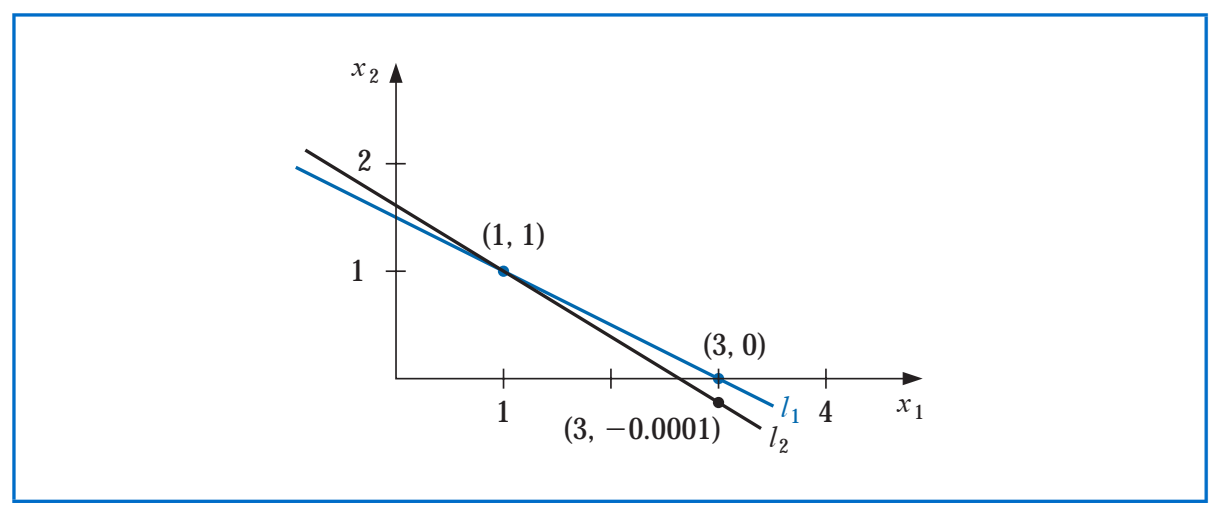
\includegraphics[width=\linewidth]{figures/figure_7.7.png}
% \caption{Minh họa cho Ví dụ 1: giao điểm của hai đường thẳng \(l_1\) và \(l_2\).}
\end{figure}

Ví dụ 1 được xây dựng có chủ đích để minh họa những khó khăn có thể xảy ra — 
và trên thực tế, thường xuyên xảy ra. 
Nếu hai đường thẳng không gần như trùng nhau, ta sẽ mong đợi rằng 
vectơ dư sẽ rất nhỏ, và khi đó nghiệm xấp xỉ sẽ chính xác.  

Trong các trường hợp tổng quát, ta không thể dựa vào hình học của hệ 
để suy ra khi nào vấn đề có thể xảy ra. 
Tuy nhiên, ta có thể thu được thông tin này bằng cách xét đến các chuẩn 
của ma trận \( A \) và ma trận nghịch đảo của nó.

\textbf{Định lý 7.27.}  
Giả sử \( \tilde{x} \) là nghiệm xấp xỉ của hệ \( A x = b \), 
\( A \) là ma trận khả nghịch, và \( r \) là vectơ dư tương ứng với \( \tilde{x} \).  
Khi đó, với mọi chuẩn (norm) tự nhiên, ta có:
\[
\|x - \tilde{x}\| \leq \|r\| \cdot \|A^{-1}\|,
\]
và nếu \( x \neq 0 \) và \( b \neq 0 \),
\[
\frac{\|x - \tilde{x}\|}{\|x\|} \leq \|A\| \cdot \|A^{-1}\| \cdot \frac{\|r\|}{\|b\|}.
\tag{7.20}
\]

\textbf{Chứng minh.}  
Vì \( r = b - A\tilde{x} = A x - A\tilde{x} \) và \( A \) khả nghịch, ta có
\( x - \tilde{x} = A^{-1} r \).  
Định lý 7.11 (trang 440) cho ta:
\[
\|x - \tilde{x}\| = \|A^{-1} r\| \leq \|A^{-1}\| \cdot \|r\|.
\]
Hơn nữa, vì \( b = A x \), nên \( \|b\| \leq \|A\| \cdot \|x\| \).  
Do đó \( 1/\|x\| \leq \|A\| / \|b\| \), và suy ra:
\[
\frac{\|x - \tilde{x}\|}{\|x\|} 
\leq \|A\| \cdot \|A^{-1}\| \cdot \frac{\|r\|}{\|b\|}.
\quad \blacksquare
\]

\subsection{Số điều kiện (Condition Numbers).}  
Bất đẳng thức trong Định lý 7.27 cho thấy rằng \( \|A^{-1}\| \) và \( \|A\| \)
cung cấp một chỉ số về mối quan hệ giữa vectơ dư và độ chính xác của nghiệm xấp xỉ.  
Trong thực tế, sai số tương đối 
\[
\frac{\|x - \tilde{x}\|}{\|x\|}
\]
là đại lượng được quan tâm nhiều nhất.  
Theo Bất đẳng thức (7.20), sai số tương đối này bị chặn trên bởi 
tích \( \|A\| \cdot \|A^{-1}\| \) nhân với sai số tương đối của vectơ dư, 
\[
\frac{\|r\|}{\|b\|}.
\]
Bất kỳ chuẩn thuận tiện nào cũng có thể được sử dụng cho phép xấp xỉ này, 
miễn là chuẩn đó được dùng nhất quán trong toàn bộ quá trình.

\textbf{Định nghĩa 7.28.}  
\textit{Số điều kiện (condition number)} của một ma trận khả nghịch \( A \)
tương ứng với một chuẩn \( \|\cdot\| \) được định nghĩa bởi:
\[
K(A) = \|A\| \cdot \|A^{-1}\|.
\]

Với ký hiệu này, các bất đẳng thức trong Định lý 7.27 có thể được viết lại thành:
\[
\|x - \tilde{x}\| \leq K(A) \frac{\|r\|}{\|A\|},
\]
và
\[
\frac{\|x - \tilde{x}\|}{\|x\|} \leq K(A) \frac{\|r\|}{\|b\|}.
\]

Với mọi ma trận khả nghịch \( A \) và chuẩn tự nhiên \( \|\cdot\| \), ta có:
\[
1 = \|I\| = \|A A^{-1}\| \leq \|A\| \cdot \|A^{-1}\| = K(A).
\]

Một ma trận được gọi là \textbf{điều kiện tốt} (well-conditioned) nếu \( K(A) \) gần 1, 
và là \textbf{kém điều kiện} (ill-conditioned) nếu \( K(A) \) lớn đáng kể hơn 1.  
Trong ngữ cảnh này, “độ điều kiện” phản ánh mức độ tin cậy rằng 
một vectơ dư nhỏ sẽ tương ứng với một nghiệm xấp xỉ đủ chính xác.

\textbf{Ví dụ 2.}  
Xác định số điều kiện của ma trận
\[
A = 
\begin{bmatrix}
1 & 2 \\
1.0001 & 2
\end{bmatrix}.
\]

\textbf{Lời giải.}  
Trong Ví dụ 1, ta thấy rằng nghiệm xấp xỉ \( (3, -0.0001)^T \) của nghiệm chính xác \( (1, 1)^T \) 
cho một vectơ dư rất nhỏ. Điều này cho thấy số điều kiện của \( A \) phải lớn.  
Ta có \( \|A\|_{\infty} = \max(|1| + |2|, |1.0001| + |2|) = 3.0001 \), 
và đây không phải là một giá trị lớn. Tuy nhiên,
\[
A^{-1} =
\begin{bmatrix}
-10000 & 10000 \\
5000.5 & -5000
\end{bmatrix},
\]
nên \( \|A^{-1}\|_{\infty} = 20000 \).  
Vì vậy, đối với chuẩn vô cực, ta có
\[
K(A) = (20000)(3.0001) = 60002.
\]
Kích thước của số điều kiện trong ví dụ này đủ lớn để cảnh báo rằng 
ta không nên đánh giá cao tính chính xác của nghiệm chỉ dựa trên độ nhỏ của vectơ dư.

Số điều kiện \( K_{\infty} \) có thể được tính trong Maple 
bằng cách sử dụng gói \texttt{LinearAlgebra} và ma trận \( A \).  
Khi đó, lệnh \texttt{ConditionNumber(A)} sẽ cho số điều kiện trong chuẩn \( l_{\infty} \).  
Ví dụ, ta có thể tính số điều kiện của ma trận \( A \) trong Ví dụ 2 bằng:
\[
A := \texttt{Matrix([[1,2],[1.0001,2]]): \ ConditionNumber(A)}
\]
và kết quả là
\[
60002.00000.
\]

Mặc dù số điều kiện của ma trận phụ thuộc hoàn toàn vào các chuẩn của ma trận và của nghịch đảo của nó, 
việc tính toán nghịch đảo chịu ảnh hưởng bởi sai số làm tròn và phụ thuộc vào độ chính xác của số học được sử dụng.  
Nếu các phép tính chỉ được thực hiện với \( t \) chữ số chính xác, 
số điều kiện xấp xỉ của ma trận \( A \) là chuẩn của \( A \) nhân với chuẩn của nghịch đảo xấp xỉ của \( A \), 
được tính bằng số học \( t \)-chữ số.  
Trên thực tế, số điều kiện cũng phụ thuộc vào phương pháp được dùng để tính nghịch đảo.  
Vì số lượng phép toán cần thiết để tính nghịch đảo có thể lớn, 
ta thường cần ước lượng số điều kiện mà không cần tính trực tiếp nghịch đảo.

Nếu ta giả sử rằng nghiệm xấp xỉ của hệ tuyến tính \( A x = b \) 
được tính bằng số học \( t \)-chữ số và phép khử Gauss, 
thì (theo [FM], trang 45–47) có thể chứng minh rằng vectơ dư \( r \) cho nghiệm xấp xỉ \( \tilde{x} \) thỏa mãn
\[
\|r\| \approx 10^{-t} \|A\| \cdot \|\tilde{x}\|.
\tag{7.21}
\]

Từ xấp xỉ này, ta có thể ước lượng \textit{số điều kiện hiệu dụng} (effective condition number) 
trong phép tính số học \( t \)-chữ số mà không cần phải tính nghịch đảo của ma trận \( A \).  
Thực tế, xấp xỉ này giả định rằng tất cả các phép toán số học trong quá trình khử Gauss 
được thực hiện bằng số học \( t \)-chữ số, 
nhưng các phép toán cần thiết để xác định vectơ dư được thực hiện bằng số học hai lần chính xác 
(tức là \( 2t \)-chữ số).  
Kỹ thuật này không làm tăng đáng kể chi phí tính toán, 
nhưng loại bỏ đáng kể mất mát độ chính xác xảy ra do việc trừ các số gần bằng nhau 
trong quá trình tính vectơ dư.

Xấp xỉ cho số điều kiện trong số học \( t \)-chữ số, ký hiệu \( K(A) \), 
có thể được rút ra từ việc xét hệ tuyến tính
\[
A y = r.
\]
Nghiệm của hệ này có thể được xấp xỉ dễ dàng, 
vì các hệ số nhân (multipliers) trong phép khử Gauss đã được tính sẵn.  
Vì vậy, ta có thể phân tích \( A \) dưới dạng \( P^T L U \) như trong Mục 5 của Chương 6.  
Trên thực tế, nghiệm xấp xỉ của hệ \( A y = r \) thỏa
\[
\tilde{y} \approx A^{-1} r = A^{-1}(b - A\tilde{x}) = A^{-1}b - A^{-1}A\tilde{x} = x - \tilde{x},
\tag{7.22}
\]
và
\[
x \approx \tilde{x} + \tilde{y}.
\]
Do đó, \( \tilde{y} \) là ước lượng cho sai số khi \( \tilde{x} \) xấp xỉ nghiệm chính xác \( x \) của hệ \( A x = b \).  
Từ các biểu thức (7.21) và (7.22), ta có:
\[
\|\tilde{y}\| \approx \|x - \tilde{x}\| \approx \|A^{-1} r\| 
\leq \|A^{-1}\| \cdot \|r\| 
\approx \|A^{-1}\| \cdot \|A\| \cdot 10^{-t} \|\tilde{x}\| 
= 10^{-t} \|\tilde{x}\| K(A).
\]

Điều này cho ta một xấp xỉ cho số điều kiện liên quan đến việc giải hệ \( A x = b \)
bằng phép khử Gauss và số học \( t \)-chữ số:
\[
K(A) \approx \frac{\|\tilde{y}\|}{\|\tilde{x}\|} \, 10^{t}.
\tag{7.23}
\]

\textbf{Minh họa.}  
Hệ tuyến tính được cho bởi
\[
\begin{bmatrix}
3.3330 & 15920 & -10.333 \\
2.2220 & 16.710 & 9.6120 \\
1.5611 & 5.1791 & 1.6852
\end{bmatrix}
\begin{bmatrix}
x_1 \\ x_2 \\ x_3
\end{bmatrix}
=
\begin{bmatrix}
15913 \\ 28.544 \\ 8.4254
\end{bmatrix}
\]
có nghiệm chính xác là \( x = (1, 1, 1)^T \).

Sử dụng phép khử Gauss với làm tròn 5 chữ số, 
ta nhận được các ma trận mở rộng:
\[
\begin{bmatrix}
3.3330 & 15920 & -10.333 & 15913 \\
0 & -10596 & 16.501 & 10580 \\
0 & -7451.4 & 6.5250 & -7444.9
\end{bmatrix}
\]
và
\[
\begin{bmatrix}
3.3330 & 15920 & -10.333 & 15913 \\
0 & -10596 & 16.501 & -10580 \\
0 & 0 & -5.0790 & -4.7000
\end{bmatrix}.
\]

Nghiệm xấp xỉ của hệ này là
\[
\tilde{x} = (1.2001,\ 0.99991,\ 0.92538)^T.
\]

Vector dư tương ứng với $\bar{x}$ được tính bằng độ chính xác kép như sau:

\[
\mathbf{r} = \mathbf{b} - A\bar{x}
\]

\[
=
\begin{bmatrix}
15913 \\[3pt]
28.544 \\[3pt]
8.4254
\end{bmatrix}
-
\begin{bmatrix}
3.3330 & 15920 & -10.333 \\[3pt]
2.2220 & 16.710 & 9.6120 \\[3pt]
1.5611 & 5.1791 & 1.6852
\end{bmatrix}
\begin{bmatrix}
1.2001 \\[3pt]
0.99991 \\[3pt]
0.92538
\end{bmatrix}
\]

\[
=
\begin{bmatrix}
15913 \\[3pt]
28.544 \\[3pt]
8.4254
\end{bmatrix}
-
\begin{bmatrix}
15913.00518 \\[3pt]
28.26987086 \\[3pt]
8.611560367
\end{bmatrix}
=
\begin{bmatrix}
-0.00518 \\[3pt]
0.27412914 \\[3pt]
-0.186160367
\end{bmatrix},
\]

do đó

\[
\|\mathbf{r}\|_\infty = 0.27413.
\]

Ước lượng cho số điều kiện được cho trong phần thảo luận trước đó được xác định bằng cách đầu tiên giải hệ $A y = r$ để tìm $\bar{y}$:

\[
\begin{bmatrix}
3.3330 & 15920 & -10.333 \\[3pt]
2.2220 & 16.710 & 9.6120 \\[3pt]
1.5611 & 5.1791 & 1.6852
\end{bmatrix}
\begin{bmatrix}
y_1 \\[3pt] y_2 \\[3pt] y_3
\end{bmatrix}
=
\begin{bmatrix}
-0.00518 \\[3pt]
0.27413 \\[3pt]
-0.18616
\end{bmatrix}.
\]

Điều này cho ta:

\[
\bar{y} = (-0.20008,\; 8.9987 \times 10^{-5},\; -0.0744607)^{T}.
\]

Sử dụng ước lượng trong phương trình (7.23) ta có:

\[
K(A) \approx \frac{\|\bar{y}\|_\infty}{\|\bar{x}\|_\infty} \times 10^{5} = \frac{0.20008}{1.2001} \times 10^{5} = 16672. \tag{7.24}
\]

Để xác định chính xác số điều kiện của $A$, trước hết ta phải tìm $A^{-1}$.  
Sử dụng số học làm tròn trong quá trình tính toán, ta có xấp xỉ sau:

\[
A^{-1} \approx
\begin{bmatrix}
-1.1701 \times 10^{-4} & -1.4983 \times 10^{-1} & 8.5416 \times 10^{-1} \\[3pt]
6.2782 \times 10^{-5} & 1.2124 \times 10^{-4} & -3.0662 \times 10^{-4} \\[3pt]
-8.6631 \times 10^{-5} & 1.3846 \times 10^{-1} & -1.9689 \times 10^{-1}
\end{bmatrix}.
\]

Định lý 7.11 ở trang 440 cho biết rằng $\|A^{-1}\|_\infty = 1.0041$ và $\|A\|_\infty = 15934$.  
Do đó, ma trận $A$ có điều kiện kém này có:

\[
K(A) = (1.0041)(15934) = 15999.
\]

Ước lượng trong (7.24) khá gần với giá trị chính xác của $K(A)$ và yêu cầu ít công sức tính toán hơn đáng kể.

Vì nghiệm thực sự là $x = (1, 1, 1)^{T}$ đã biết cho hệ này, ta có thể tính được rằng

\[
\|\mathbf{x} - \bar{\mathbf{x}}\|_\infty = 0.2001
\quad \text{và} \quad
\frac{\|\mathbf{x} - \bar{\mathbf{x}}\|_\infty}{\|\mathbf{x}\|_\infty}
= \frac{0.2001}{1} = 0.2001.
\]

Các giới hạn sai số được nêu trong Định lý 7.27 cho các giá trị này là

\[
\frac{\|\mathbf{x} - \bar{\mathbf{x}}\|_\infty}{\|\mathbf{x}\|_\infty}
\leq K(A) \frac{\|\mathbf{r}\|_\infty}{\|A\|_\infty}
= \frac{(15999)(0.27413)}{15934} = 0.27525
\]

và

\[
\frac{\|\mathbf{x} - \bar{\mathbf{x}}\|_\infty}{\|\mathbf{x}\|_\infty}
\leq K(A) \frac{\|\mathbf{r}\|_\infty}{\|\mathbf{b}\|_\infty}
= \frac{(15999)(0.27413)}{15913} = 0.27561.
\]

\subsection{Tinh chỉnh lặp (Iterative Refinement)}

Trong Phương trình (7.22), ta đã sử dụng ước lượng $\bar{y} \approx \mathbf{x} - \bar{\mathbf{x}}$, trong đó $\bar{y}$ là nghiệm xấp xỉ của hệ tuyến tính $A y = \mathbf{r}$.  
Nói chung, $\bar{\mathbf{x}} + \bar{y}$ là một xấp xỉ chính xác hơn cho nghiệm của hệ tuyến tính $A \mathbf{x} = \mathbf{b}$ so với xấp xỉ ban đầu $\bar{\mathbf{x}}$.  
Phương pháp sử dụng giả định này được gọi là \textit{tinh chỉnh lặp} (\textit{iterative refinement}) hay \textit{cải thiện lặp} (\textit{iterative improvement}), và bao gồm việc thực hiện nhiều phép lặp trên hệ có vế phải là vector dư, để có được các xấp xỉ liên tiếp cho đến khi đạt được kết quả có độ chính xác thỏa đáng.

Nếu quá trình này được áp dụng bằng số học có $t$ chữ số và nếu $K_{\infty}(A) \approx 10^{q}$, thì sau $k$ vòng lặp tinh chỉnh lặp, nghiệm thu được sẽ có xấp xỉ bằng số chữ số nhỏ hơn giữa $t$ và $t(k - q)$ chữ số chính xác.  
Nếu hệ có điều kiện tốt, một hoặc hai lần lặp thường đủ để xác nhận rằng nghiệm là chính xác.  
Có khả năng cải thiện đáng kể trên các hệ có điều kiện kém, trừ khi ma trận $A$ có điều kiện quá tệ đến mức $K_{\infty}(A) > 10^{t}$.  
Trong tình huống đó, nên sử dụng độ chính xác cao hơn cho các phép tính.

\subsection*{Thuật toán 7.4 — Tinh chỉnh lặp (Iterative Refinement)}

\textbf{Mục tiêu:}  
Xấp xỉ nghiệm cho hệ tuyến tính $A\mathbf{x} = \mathbf{b}$.

\textbf{Dữ liệu đầu vào:}
\begin{itemize}
    \item Số lượng phương trình và ẩn $n$;
    \item Các phần tử $a_{ij},\; 1 \leq i, j \leq n$ của ma trận $A$;
    \item Các phần tử $b_i,\; 1 \leq i \leq n$ của $\mathbf{b}$;
    \item Số lần lặp tối đa $N$;
    \item Ngưỡng sai số $TOL$;
    \item Số chữ số chính xác $t$.
\end{itemize}

\textbf{Dữ liệu đầu ra:}  
Nghiệm xấp xỉ $\mathbf{x} = (x_1, x_2, \dots, x_n)^{T}$ hoặc thông báo rằng số lần lặp vượt quá giới hạn, kèm theo giá trị xấp xỉ của số điều kiện $\text{COND} \approx K_{\infty}(A)$.


Giải hệ $A\mathbf{x} = \mathbf{b}$ cho $x_1, \dots, x_n$ bằng phương pháp khử Gauss, lưu các hệ số nhân $m_{ij},\; j = i+1, i+2, \dots, n;\; i = 1, 2, \dots, n-1$ và lưu lại các phép hoán đổi hàng.

\begin{enumerate}[label=\textbf{Step \arabic*:}, leftmargin=2.5em]

\item Đặt $k = 1$.

\item Trong khi $(k \leq N)$ thì thực hiện các Bước 3–9.

\item Với $i = 1, 2, \dots, n$ (tính $\mathbf{r}$):
\[
r_i = b_i - \sum_{j=1}^{n} a_{ij}x_j.
\]
(Thực hiện các phép tính bằng số học độ chính xác kép.)

\item Giải hệ tuyến tính $A y = \mathbf{r}$ bằng phương pháp khử Gauss theo cùng thứ tự như ở Bước 0.

\item Với $i = 1, \dots, n$, đặt $x_i := x_i + y_i$.

\item Nếu $k = 1$ thì đặt 
\[
\text{COND} = \frac{\|\mathbf{y}\|_{\infty}}{\|\mathbf{x}\|_{\infty}} \times 10^{t}.
\]

\item Nếu $\|\mathbf{x} - \bar{\mathbf{x}}\|_{\infty} < TOL$ thì  
\textbf{OUTPUT} $(\mathbf{x})$;  
\textbf{OUTPUT} $(\text{COND});$  
\textbf{(Thuật toán đã hội tụ thành công.)}  
\textbf{STOP.}

\item Đặt $k = k + 1$.

\item Với $i = 1, \dots, n$, đặt $x_i := x_i$.

\item OUTPUT (‘Số lần lặp tối đa đã bị vượt quá’); \\
OUTPUT (COND); \\
\textit{(Thuật toán không thành công.)} \\
STOP.

\end{enumerate}


Nếu sử dụng số học $t$-chữ số, một quy tắc dừng được khuyến nghị trong Bước 7 là lặp lại cho đến khi
\[
|y_i^{(k)}| \leq 10^{-t}, \quad \text{với mỗi } i = 1, 2, \dots, n.
\]

\subsection*{Minh họa}

Trong ví dụ trước, ta đã tìm được nghiệm xấp xỉ cho hệ tuyến tính
\[
\begin{bmatrix}
3.3330 & 15920 & -10.333 \\[3pt]
2.2220 & 16.710 & 9.6120 \\[3pt]
1.5611 & 5.1791 & 1.6852
\end{bmatrix}
\begin{bmatrix}
x_1 \\[3pt]
x_2 \\[3pt]
x_3
\end{bmatrix}
=
\begin{bmatrix}
15913 \\[3pt]
28.544 \\[3pt]
8.4254
\end{bmatrix}
\]
bằng cách sử dụng số học 5 chữ số và khử Gauss, thu được
\[
\bar{\mathbf{x}}^{(1)} = (1.2001,\, 0.99991,\, 0.92538)^{T}.
\]

Nghiệm của hệ $A y = \mathbf{r}^{(1)}$ được tính là
\[
\bar{\mathbf{y}}^{(1)} = (-0.20008,\, 8.9987 \times 10^{-5},\, -0.0744607)^{T}.
\]

Theo Bước 5 của thuật toán này, ta có
\[
\bar{\mathbf{x}}^{(2)} = \bar{\mathbf{x}}^{(1)} + \bar{\mathbf{y}}^{(1)} = (1.0000,\, 1.00000,\, 0.99999)^{T}.
\]

Sai số thực tế trong xấp xỉ này là
\[
\|\mathbf{x} - \bar{\mathbf{x}}^{(2)}\|_{\infty} = 1 \times 10^{-5}.
\]

Sử dụng quy tắc dừng được đề xuất cho thuật toán, ta tính
\[
\mathbf{r}^{(2)} = \mathbf{b} - A \bar{\mathbf{x}}^{(2)},
\]
và giải hệ $A y^{(2)} = \mathbf{r}^{(2)}$, thu được
\[
\bar{\mathbf{y}}^{(2)} = (1.5002 \times 10^{-9},\, 2.0951 \times 10^{-10},\, -1.0000 \times 10^{-5})^{T}.
\]

Vì $\|\bar{\mathbf{y}}^{(2)}\|_{\infty} \leq 10^{-5}$, ta kết luận rằng
\[
\bar{\mathbf{x}}^{(3)} = \bar{\mathbf{x}}^{(2)} + \bar{\mathbf{y}}^{(2)} = (1.0000,\, 1.0000,\, 1.0000)^{T}
\]
là nghiệm đủ chính xác — và điều đó hoàn toàn đúng.

\vspace{0.5em}

Trong toàn bộ phần này, ta đã giả định rằng trong hệ tuyến tính $A\mathbf{x} = \mathbf{b}$, cả $A$ và $\mathbf{b}$ đều được biểu diễn chính xác.  
Trên thực tế, các phần tử $a_{ij}$ và $b_j$ có thể bị thay đổi hoặc nhiễu đi một lượng nhỏ $\delta a_{ij}$ và $\delta b_j$, khiến cho hệ tuyến tính trở thành:

\[
(A + \delta A)\mathbf{x} = \mathbf{b} + \delta \mathbf{b}.
\]

Hệ này được giải để tìm $\mathbf{x}$ trong phương trình $A\mathbf{x} = \mathbf{b}$.  
Thông thường, nếu $\|\delta A\|$ và $\|\delta \mathbf{b}\|$ đều nhỏ (cỡ $10^{-t}$), thì số học $t$-chữ số sẽ cho ra một nghiệm $\bar{\mathbf{x}}$ mà sai số $\|\mathbf{x} - \bar{\mathbf{x}}\|$ cũng tương ứng nhỏ.  
Tuy nhiên, trong trường hợp các hệ có điều kiện kém, ta đã thấy rằng ngay cả khi $A$ và $\mathbf{b}$ được biểu diễn chính xác, các lỗi làm tròn cũng có thể khiến $\|\mathbf{x} - \bar{\mathbf{x}}\|$ trở nên lớn. Định lý tiếp theo liên hệ sự nhiễu loạn (sai lệch) của các hệ phương trình tuyến tính với số điều kiện (condition number) của một ma trận. Chứng minh của kết quả này có thể được tìm thấy trong [Or2], trang 33.


\subsection*{Định lý 7.29}

Giả sử \(A\) là khả nghịch và
\[
\|\delta A\| < \frac{1}{\|A^{-1}\|}.
\]

Nghiệm \(\tilde{x}\) của hệ
\[
(A + \delta A)\tilde{x} = \mathbf{b} + \delta\mathbf{b}
\]
xấp xỉ nghiệm \(\mathbf{x}\) của \(A\mathbf{x} = \mathbf{b}\) với ước lượng sai số

\[
\frac{\|\mathbf{x} - \tilde{\mathbf{x}}\|}{\|\mathbf{x}\|}
\le
\frac{K(A)\,\|A\|}{\|A\| - K(A)\|\delta A\|}
\left(
\frac{\|\delta\mathbf{b}\|}{\|\mathbf{b}\|}
+
\frac{\|\delta A\|}{\|A\|}
\right).
\tag{7.25}
\]

Ước lượng trong bất đẳng thức (7.25) phát biểu rằng nếu ma trận \(A\) có điều kiện tốt (tức là \(K(A)\) không quá lớn), thì các thay đổi nhỏ trong \(A\) và \(\mathbf{b}\) sẽ tạo ra những thay đổi tương ứng nhỏ trong nghiệm \(\mathbf{x}\). Ngược lại, nếu \(A\) có điều kiện kém, thì những thay đổi nhỏ trong \(A\) và \(\mathbf{b}\) có thể gây ra thay đổi lớn trong \(\mathbf{x}\).

Định lý này không phụ thuộc vào phương pháp số cụ thể được dùng để giải \(A\mathbf{x} = \mathbf{b}\).  
Người ta có thể chứng minh, bằng phân tích sai số ngược (backward error analysis), rằng nếu khử Gauss có pivot được sử dụng để giải \(A\mathbf{x} = \mathbf{b}\) trong số học có \(t\) chữ số, thì nghiệm số \(\tilde{\mathbf{x}}\) là nghiệm thực của một hệ tuyến tính dạng:

\[
(A + \delta A)\tilde{\mathbf{x}} = \mathbf{b},
\qquad\text{trong đó}\quad
\|\delta A\|_\infty \le f(n)10^{1-t}\max_{i,j,k}|a_{ij}^{(k)}|,
\]

với một hàm số \(f(n)\). Wilkinson nhận thấy rằng trong thực tế \(f(n)\approx n\) và, trong trường hợp xấu nhất, \(f(n) \le 1.01(n^3 + 3n^2)\).




% Chapter 9
\chapter*{Kết luận}
\label{chap:conclusion}

Trong quá trình nghiên cứu, chúng ta đã lần lượt tiếp cận và phân tích 
nhiều phương pháp lặp khác nhau được sử dụng trong giải tích số — từ các kỹ thuật tìm nghiệm của phương trình phi tuyến một ẩn đến các phương pháp lặp giải hệ phương trình tuyến tính nhiều ẩn.  
Những phương pháp này không chỉ đóng vai trò là công cụ tính toán hiệu quả, mà còn thể hiện tư tưởng nền tảng của toán học tính toán hiện đại: 
\textit{dùng quá trình xấp xỉ có kiểm soát để tiệm cận dần đến nghiệm chính xác}.

Ở phần đầu, các phương pháp như Bisection, Fixed-Point Iteration, Newton và các biến thể của nó cho thấy sự tiến hóa từ những kỹ thuật đơn giản, ổn định đến những phương pháp có tốc độ hội tụ nhanh và độ chính xác cao hơn.
Phân tích sai số và bậc hội tụ giúp ta hiểu rõ hơn vì sao cùng một bài toán, các phương pháp khác nhau lại cho kết quả và tốc độ tiệm cận khác nhau.  
Những kỹ thuật tăng tốc hội tụ như Aitken’s $\Delta^2$ Process và Steffensen’s Method minh chứng cho khả năng kết hợp giữa tính hiệu quả và sự tinh gọn về mặt thuật toán, cho phép đạt được tốc độ hội tụ bậc hai mà không cần đạo hàm — một bước tiến quan trọng trong thiết kế các phương pháp lặp hiện đại.

Phần sau mở rộng các tư tưởng đó sang lĩnh vực đại số tuyến tính,
nơi các hệ phương trình lớn xuất hiện phổ biến trong kỹ thuật, vật lý và mô phỏng số.
Các phương pháp Jacobi, Gauss–Seidel và SOR (Successive Over-Relaxation) 
thể hiện cách tiếp cận linh hoạt trong việc giải hệ phương trình tuyến tính thông qua quá trình lặp dần, đồng thời cung cấp cơ chế kiểm soát sai số và tăng tốc hội tụ dựa trên cấu trúc ma trận và tham số thư giãn thích hợp.
Các kỹ thuật đánh giá sai số và hiệu chỉnh nghiệm lặp (Iterative Refinement)cũng được giới thiệu như một phần không thể thiếu để đảm bảo tính ổn định và độ chính xác của kết quả tính toán.

Tổng thể, các nội dung được trình bày trong tiểu luận 
đã cho thấy mối liên hệ chặt chẽ giữa lý thuyết và thực hành trong giải tích số.  
Các phương pháp lặp không chỉ là công cụ giải toán thuần túy, 
mà còn là nền tảng cho hàng loạt thuật toán hiện đại 
trong tối ưu hóa, học máy, mô phỏng động lực học và tính toán khoa học.



% Appendix A
\newpage
\chapter*{PHỤ LỤC}




\nocite{*}
\bibliographystyle{IEEEtranS}
\bibliography{ref}

\end{document}
